\section{\textbf{APPENDIX ELLIPSE CURVE}} \label{APPENDIX ELLIPSE CURVE}


\subsection       {Plot of Ellipse curve
	[\ref  {01-img-Plot of Ellipse curve.pdf} ] }
\label{ssec-01-img-Plot of Ellipse curve.pdf}

\subsection       {Ellipse Radius of Curvature
[\ref      {02-img-Ellipse Radius of Curvature.pdf}] }
\label{ssec-02-img-Ellipse Radius of Curvature.pdf}

\subsection       {Ellipse Validation in LinuxCNC
[\ref      {03-img-Ellipse-Validation-in-LinuxCNC.png} ] }
\label{ssec-03-img-Ellipse-Validation-in-LinuxCNC.png}

\subsection     {Ellipse Direction of Travel 3D
[\ref      {04-img-Ellipse Direction of Travel 3D.pdf} ] }
\label{ssec-04-img-Ellipse Direction of Travel 3D.pdf}

\subsection       {Ellipse First and Second Order Taylor's Approx
[\ref      {05-img-Ellipse-First-and-Second-Order-Taylors-Approx.pdf}] }
\label{ssec-05-img-Ellipse-First-and-Second-Order-Taylors-Approx.pdf}

\subsection       {Ellipse First minus Second Order Taylor's Approx
[\ref      {06-img-Ellipse-First-minus-Second-Order-Taylors-Approx.pdf}] }
\label{ssec-06-img-Ellipse-First-minus-Second-Order-Taylors-Approx.pdf}

\subsection       {Ellipse Separate First and Second Order Taylor's Approx
[\ref      {07-img-Ellipse-Separation-First-and-Second-Order-Taylors-Approx.pdf} ] }
\label{ssec-07-img-Ellipse-Separation-First-and-Second-Order-Taylors-Approx.pdf}

\subsection       {Ellipse Separation SAL and SCL
[\ref      {08-img-Ellipse-Separation-SAL-and-SCL.pdf}] }
\label{ssec-08-img-Ellipse-Separation-SAL-and-SCL.pdf}

\subsection       {Ellipse Chord-error in close view 2 scales
[\ref      {09-img-Ellipse-Chord-error-in-close-view-2-scales.pdf}] }
\label{ssec-09-img-Ellipse-Chord-error-in-close-view-2-scales.pdf}

\subsection       {Ellipse Four Components Feedrate Limit
[\ref      {10-img-Ellipse-Four-Components-Feedrate-Limit.pdf} ] }
\label{ssec-10-img-Ellipse-Four-Components-Feedrate-Limit.pdf}

\subsection    {Ellipse FrateCommand FrateLimit and Curr-Frate
[\ref      {11-img-Ellipse-FrateCommand-FrateLimit-and-Curr-Frate.pdf}] }
\label{ssec-11-img-Ellipse-FrateCommand-FrateLimit-and-Curr-Frate.pdf}

\subsection     {Ellipse FeedRateLimit minus CurrFeedRate
[\ref      {12-img-Ellipse-FeedRateLimit-minus-CurrFeedRate.pdf} ] }
\label{ssec-12-img-Ellipse-FeedRateLimit-minus-CurrFeedRate.pdf}

\subsection     {Ellipse FC20-Nominal X and Y Feedrate Profiles
[\ref      {13-img-Ellipse-FC20-Nominal-X-and-Y-Feedrate-Profiles.pdf} ] }
\label{ssec-13-img-Ellipse-FC20-Nominal-X-and-Y-Feedrate-Profiles.pdf}

\subsection     {Ellipse FC20 Nominal Tangential Acceleration
[\ref      {14-img-Ellipse-FC20-Nominal-Tangential-Acceleration.pdf} ] }
\label{ssec-14-img-Ellipse-FC20-Nominal-Tangential-Acceleration.pdf}

\subsection     {Ellipse FC20 Nominal Rising S-Curve Profile
[\ref      {15-img-Ellipse-FC20-Nominal-Rising-S-Curve-Profile.pdf} ] }
\label{ssec-15-img-Ellipse-FC20-Nominal-Rising-S-Curve-Profile.pdf}

\subsection     {Ellipse FC20 Nominal Falling S-Curve Profile
[\ref      {16-img-Ellipse-FC20-Nominal-Falling-S-Curve-Profile.pdf}] }
\label{ssec-16-img-Ellipse-FC20-Nominal-Falling-S-Curve-Profile.pdf}

\subsection       {Ellipse FC10 Colored Feedrate Profile data ngcode
[\ref      {17-img-Ellipse-FC10-Colored-Feedrate-Profile-data_ngcode.png} ] }
\label{ssec-17-img-Ellipse-FC10-Colored-Feedrate-Profile-data_ngcode.png}

\subsection       {Ellipse FC20 Colored Feedrate Profile data ngcode
[\ref      {18-img-Ellipse-FC20-Colored-Feedrate-Profile-data_ngcode.png} ] }
\label{ssec-18-img-Ellipse-FC20-Colored-Feedrate-Profile-data_ngcode.png}

Continue ...\\

\subsection       {Ellipse FC30 Colored Feedrate Profile data ngcode
[\ref      {19-img-Ellipse-FC30-Colored-Feedrate-Profile-data_ngcode.png} ] }
\label{ssec-19-img-Ellipse-FC30-Colored-Feedrate-Profile-data_ngcode.png}

\subsection       {Ellipse FC40 Colored Feedrate Profile data ngcode
[\ref      {20-img-Ellipse-FC40-Colored-Feedrate-Profile-data_ngcode.png} ] }
\label{ssec-20-img-Ellipse-FC40-Colored-Feedrate-Profile-data_ngcode.png}

\subsection       {Ellipse FC10 Tangential Acceleration
[\ref      {21-img-Ellipse-FC10-Tangential-Acceleration.pdf}] }
\label{ssec-21-img-Ellipse-FC10-Tangential-Acceleration.pdf}

\subsection       {Ellipse FC20 Tangential Acceleration
[\ref      {22-img-Ellipse-FC20-Tangential-Acceleration.pdf}] }
\label{ssec-22-img-Ellipse-FC20-Tangential-Acceleration.pdf}

\subsection       {Ellipse FC30 Tangential Acceleration
[\ref      {23-img-Ellipse-FC30-Tangential-Acceleration.pdf}] }
\label{ssec-23-img-Ellipse-FC30-Tangential-Acceleration.pdf}

\subsection       {Ellipse FC40 Tangential Acceleration
[\ref      {24-img-Ellipse-FC40-Tangential-Acceleration.pdf}] }
\label{ssec-24-img-Ellipse-FC40-Tangential-Acceleration.pdf}

\subsection       {Ellipse FC20 Nominal Separation NAL and NCL
[\ref      {25-img-Ellipse-FC20-Nominal-Separation-NAL-and-NCL.pdf}] }
\label{ssec-25-img-Ellipse-FC20-Nominal-Separation-NAL-and-NCL.pdf}

\subsection       {Ellipse SAL minus SCL for FC10 FC20 FC30 FC40
[\ref      {26-img-Ellipse-Difference-SAL-minus-SCL-for-FC10-FC20-FC30-FC40.pdf}] }
\label{ssec-26-img-Ellipse-Difference-SAL-minus-SCL-for-FC10-FC20-FC30-FC40.pdf}


\subsection       {Ellipse FC10 FrateCmd CurrFrate X-Frate Y-Frate
[\ref      {27-img-Ellipse-FC10-FrateCmd-CurrFrate-X-Frate-Y-Frate.pdf}] }
\label{ssec-27-img-Ellipse-FC10-FrateCmd-CurrFrate-X-Frate-Y-Frate.pdf}

\subsection       {Ellipse FC20 FrateCmd CurrFrate X-Frate Y-Frate
[\ref      {28-img-Ellipse-FC20-FrateCmd-CurrFrate-X-Frate-Y-Frate.pdf}] }
\label{ssec-28-img-Ellipse-FC20-FrateCmd-CurrFrate-X-Frate-Y-Frate.pdf}

\subsection       {Ellipse FC30 FrateCmd CurrFrate X-Frate Y-Frate
[\ref      {29-img-Ellipse-FC30-FrateCmd-CurrFrate-X-Frate-Y-Frate.pdf}] }
\label{ssec-29-img-Ellipse-FC30-FrateCmd-CurrFrate-X-Frate-Y-Frate.pdf}

\subsection       {Ellipse FC40 FrateCmd CurrFrate X-Frate Y-Frate
[\ref      {30-img-Ellipse-FC40-FrateCmd-CurrFrate-X-Frate-Y-Frate.pdf}] }
\label{ssec-30-img-Ellipse-FC40-FrateCmd-CurrFrate-X-Frate-Y-Frate.pdf}

\subsection       {Ellipse FC10 Four Components FeedrateLimit
[\ref      {31-img-Ellipse-FC10-Four-Components-FeedrateLimit.pdf}] }
\label{ssec-31-img-Ellipse-FC10-Four-Components-FeedrateLimit.pdf}

\subsection       {Ellipse FC20 Four Components FeedrateLimit
[\ref      {32-img-Ellipse-FC20-Four-Components-FeedrateLimit.pdf}] }
\label{ssec-32-img-Ellipse-FC20-Four-Components-FeedrateLimit.pdf}

\subsection       {Ellipse FC30 Four Components FeedrateLimit
[\ref      {33-img-Ellipse-FC30-Four-Components-FeedrateLimit.pdf}] }
\label{ssec-33-img-Ellipse-FC30-Four-Components-FeedrateLimit.pdf}

\subsection       {Ellipse FC40 Four Components FeedrateLimit
[\ref      {34-img-Ellipse-FC40-Four-Components-FeedrateLimit.pdf}]}
\label{ssec-34-img-Ellipse-FC40-Four-Components-FeedrateLimit.pdf}

\subsection       {Ellipse Histogram Points FC10 FC20 FC30 FC40
[\ref      {35-img-Ellipse-Histogram-Points-FC10-FC20-FC30-FC40.pdf}] }
\label{ssec-35-img-Ellipse-Histogram-Points-FC10-FC20-FC30-FC40.pdf}

\subsection    {Ellipse Table distribution of interpolated points
[\ref      {tab-Ellipse Table distribution of interpolated points}] }
\label{ssec-tab-Ellipse Table distribution of interpolated points}

\subsection         {Ellipse Table FC10-20-30-40 Run Performance data
[\ref      {tab-app4-Ellipse-Table-FC10-20-30-40-Run-Performance-data}] }
\label{ssec-tab-app4-Ellipse-Table-FC10-20-30-40-Run-Performance-data}


%% =====================================================
%% =====================================================
\clearpage
\pagebreak

\begin{figure}
	\caption     {Plot of Ellipse curve}
	\label{01-img-Plot of Ellipse curve.pdf}
	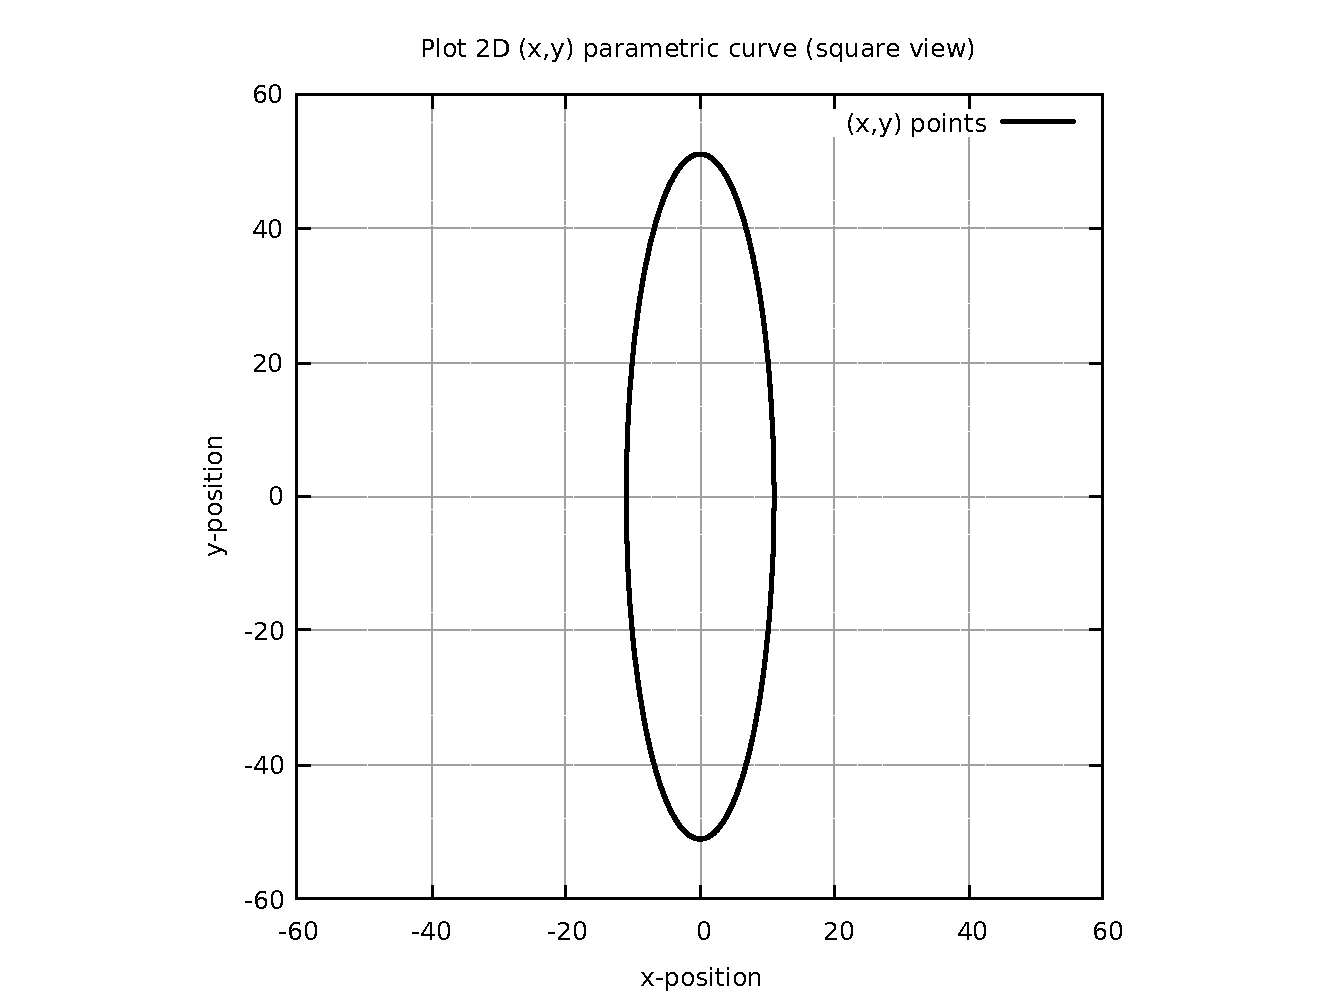
\includegraphics[width=1.00\textwidth]{Chap4/appendix/app-Ellipse/plots/01-img-Plot of Ellipse curve.pdf}
\end{figure}	


\begin{figure}
	\caption     {Ellipse Radius of Curvature}
	\label{02-img-Ellipse Radius of Curvature.pdf}
	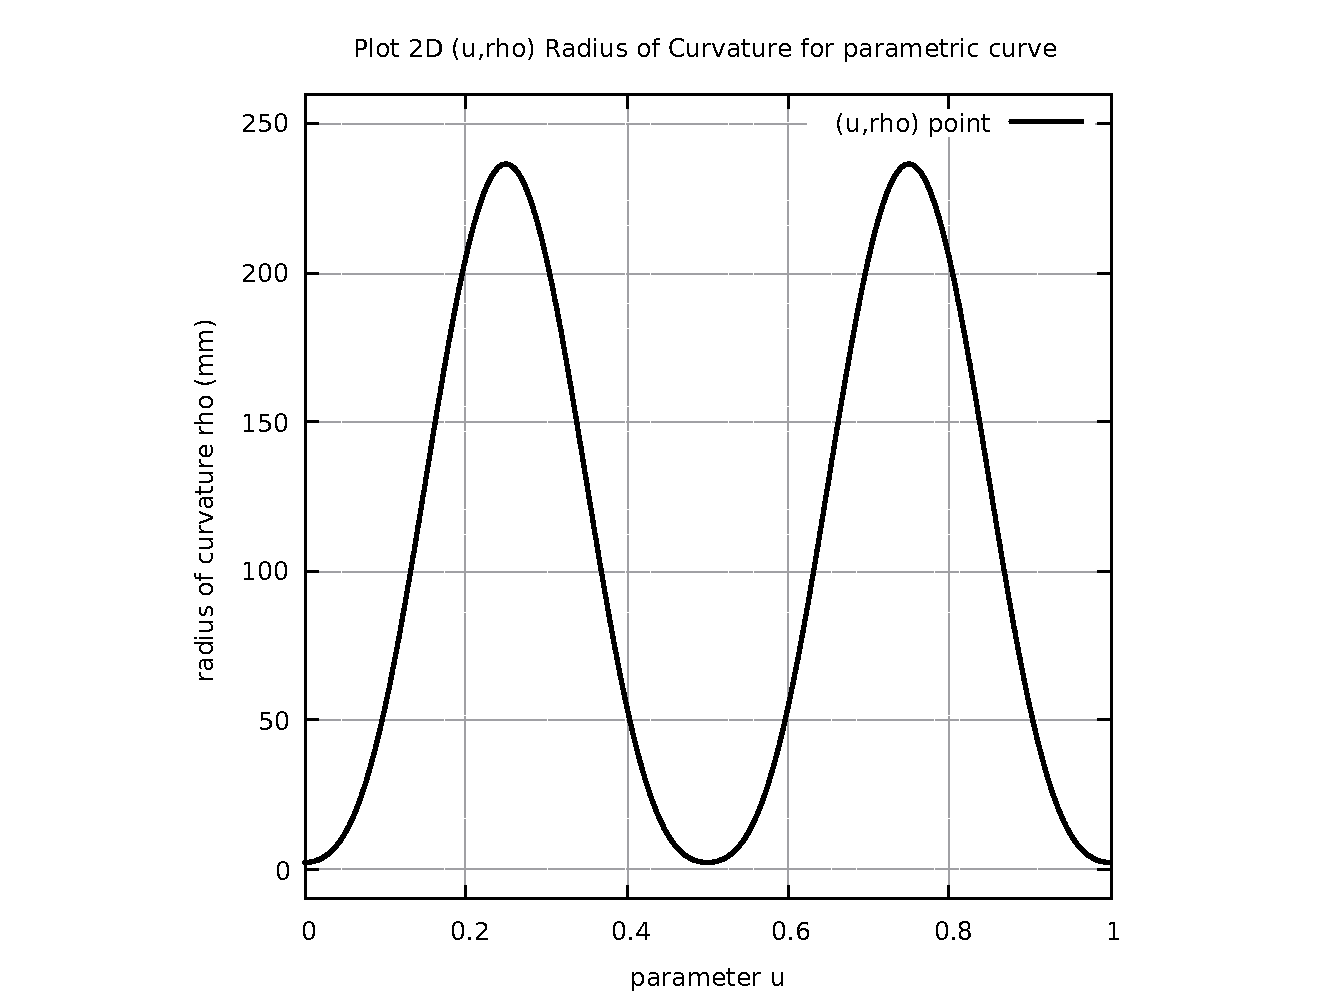
\includegraphics[width=1.00\textwidth]{Chap4/appendix/app-Ellipse/plots/02-img-Ellipse Radius of Curvature.pdf} 
\end{figure}	


%% ==================================================
\clearpage
\pagebreak

\begin{figure}
	\caption     {Ellipse Validation in LinuxCNC}
	\label{03-img-Ellipse-Validation-in-LinuxCNC.png}
	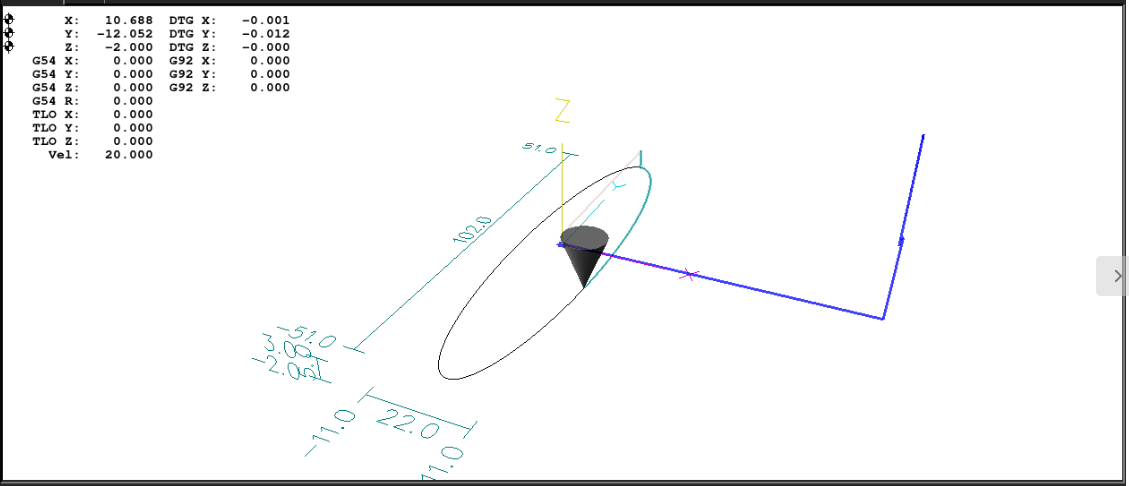
\includegraphics[width=1.00\textwidth]{Chap4/appendix/app-Ellipse/plots/03-img-Ellipse-Validation-in-LinuxCNC.png}
\end{figure}


\begin{figure}
	\caption     {Ellipse Direction of Travel 3D}
	\label{04-img-Ellipse Direction of Travel 3D.pdf}
	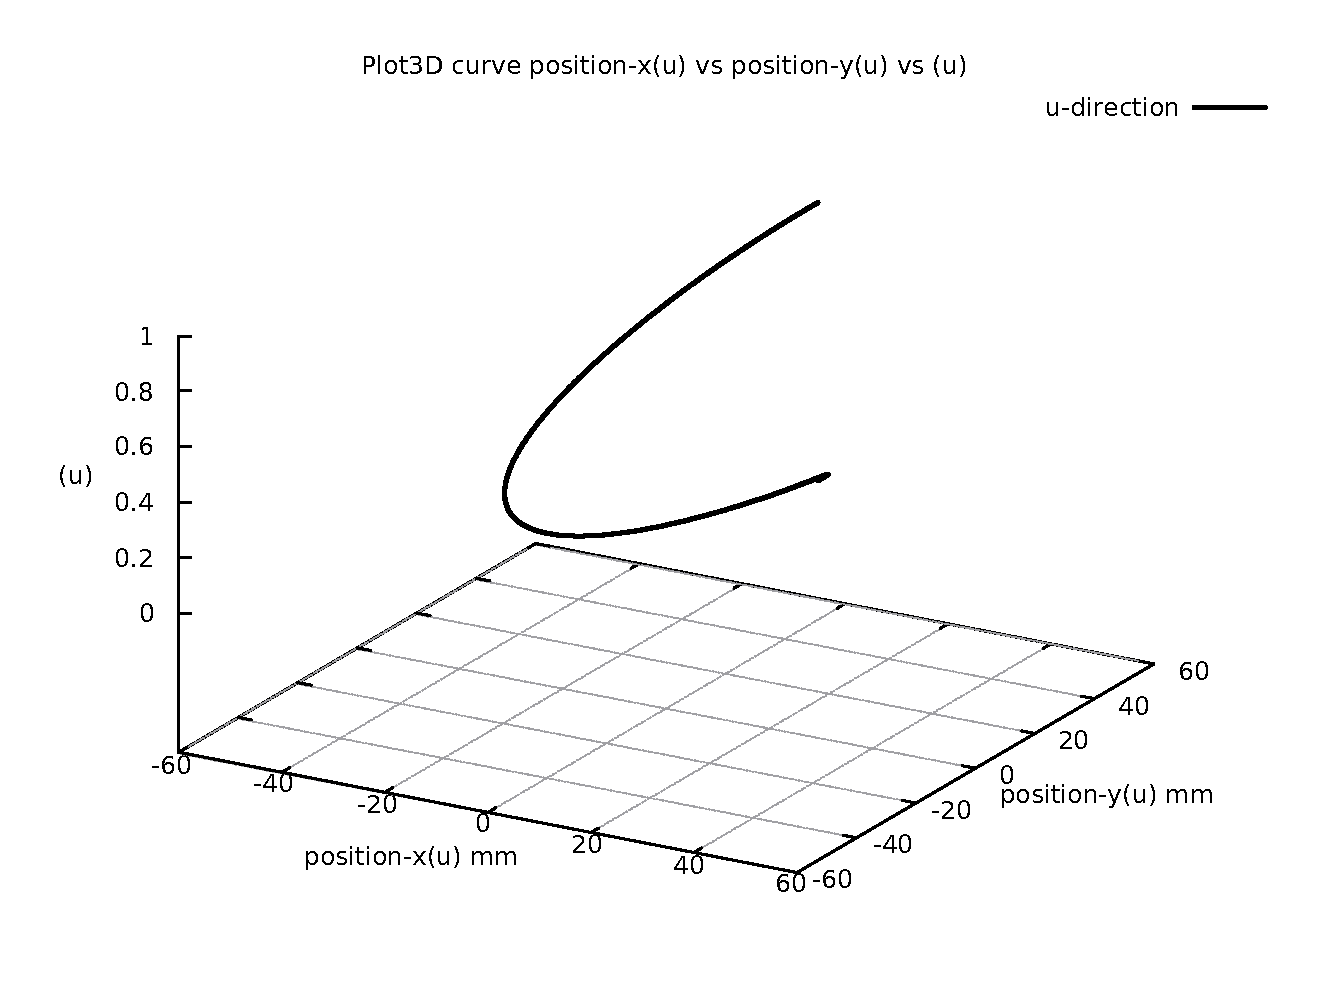
\includegraphics[width=1.00\textwidth]{Chap4/appendix/app-Ellipse/plots/04-img-Ellipse Direction of Travel 3D.pdf}
\end{figure}

%% ==================================================
\clearpage
\pagebreak

\begin{figure}
	\caption     {Ellipse First and Second Order Taylor's Approximation}
	\label{05-img-Ellipse-First-and-Second-Order-Taylors-Approx.pdf}
	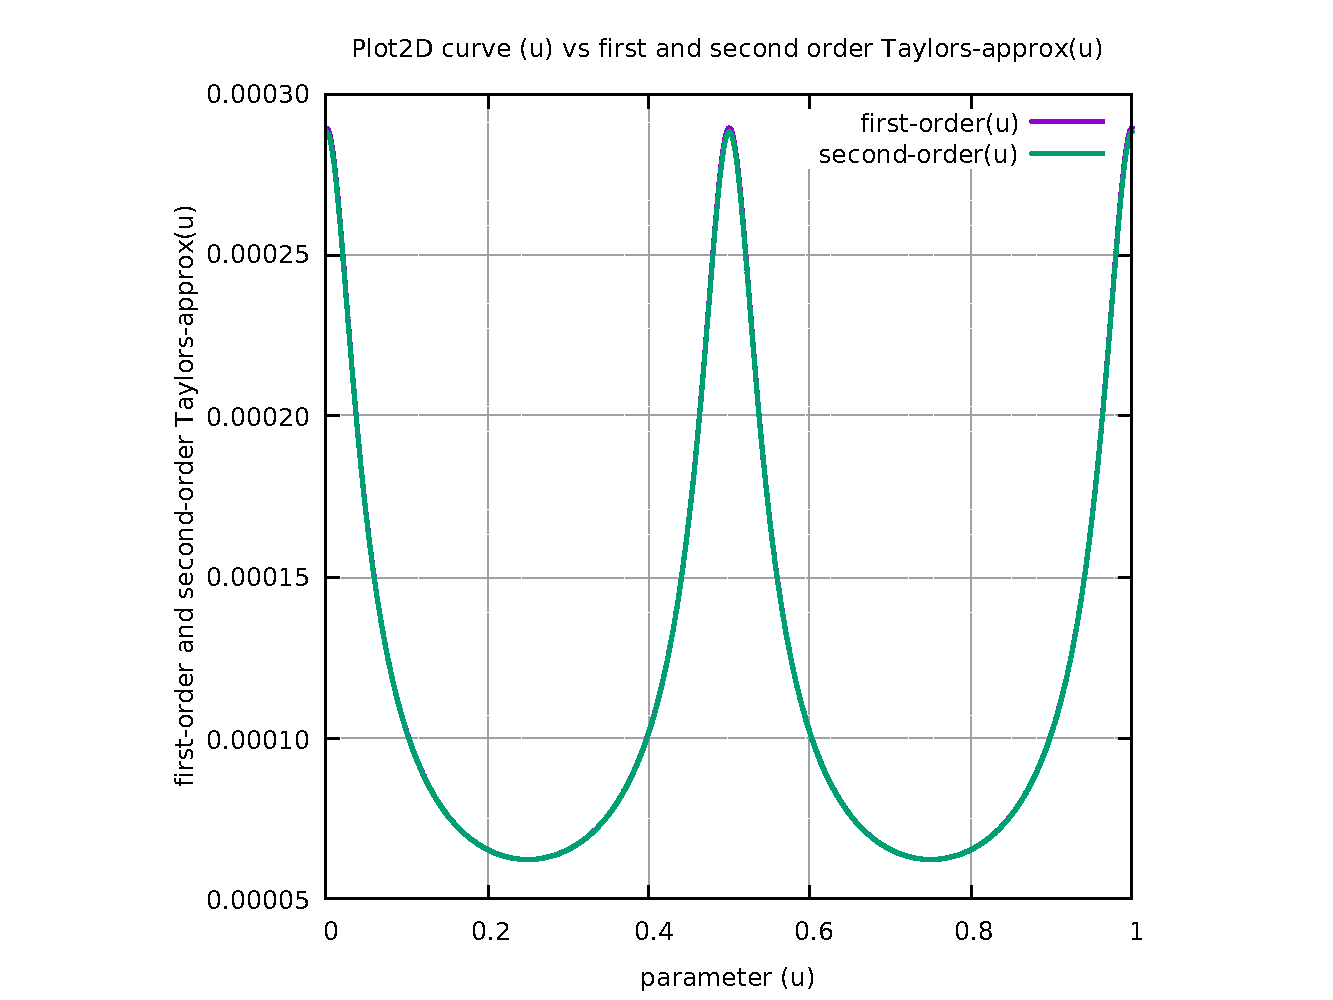
\includegraphics[width=1.00\textwidth]{Chap4/appendix/app-Ellipse/plots/05-img-Ellipse-First-and-Second-Order-Taylors-Approx.pdf}
\end{figure}


\begin{figure}
	\caption     {Ellipse First minus Second Order Taylor's Approximation}
	\label{06-img-Ellipse-First-minus-Second-Order-Taylors-Approx.pdf}
	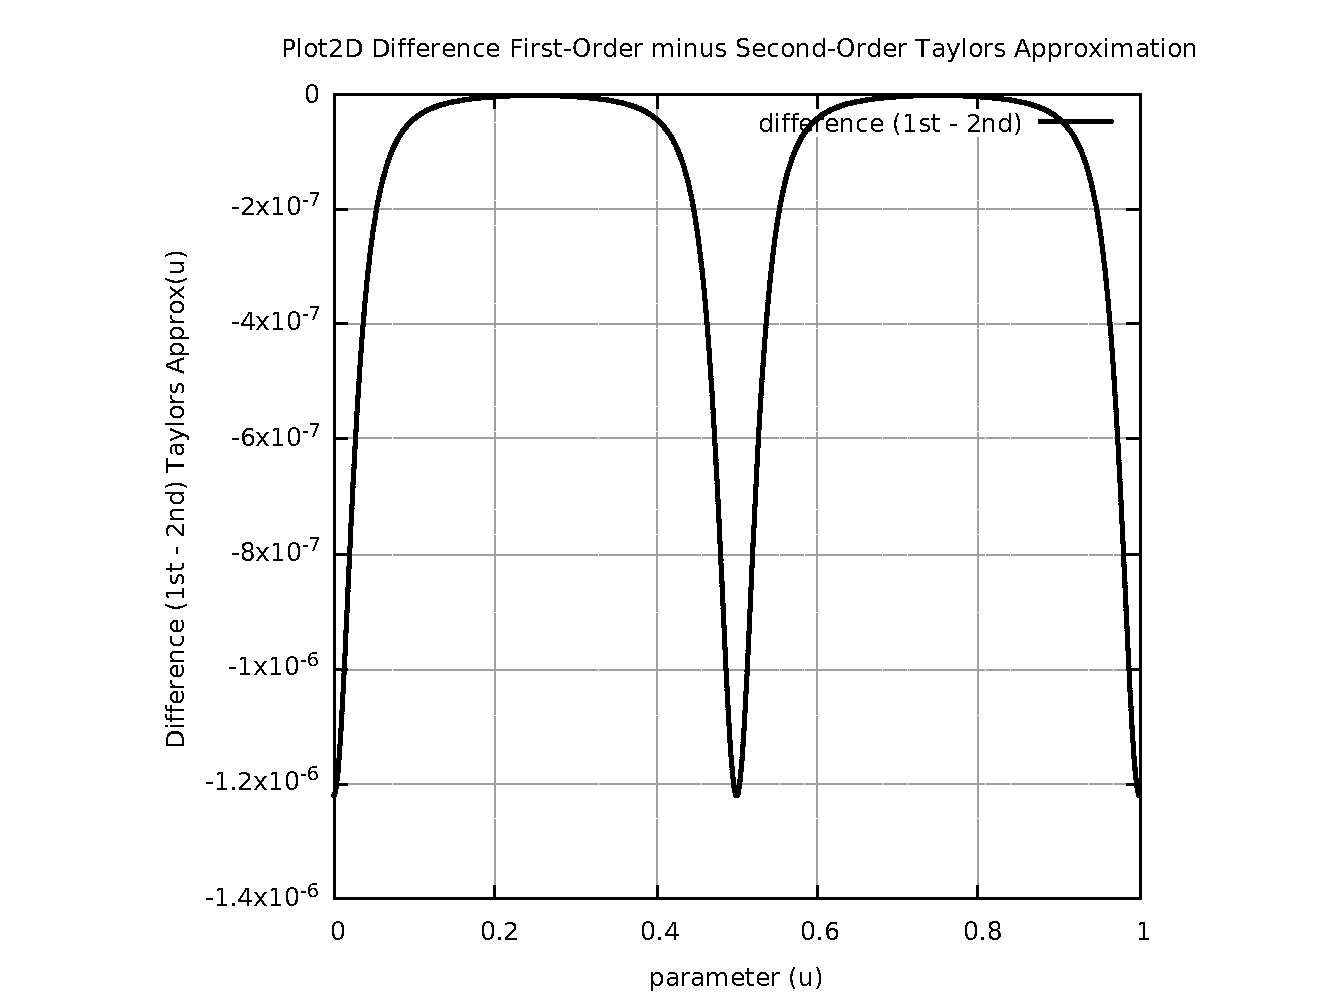
\includegraphics[width=1.00\textwidth]{Chap4/appendix/app-Ellipse/plots/06-img-Ellipse-First-minus-Second-Order-Taylors-Approx.pdf}
\end{figure}

%% ==================================================
\clearpage
\pagebreak

\begin{figure}
	\caption     {Ellipse Separation First and Second Order Taylor's Approximation}
	\label{07-img-Ellipse-Separation-First-and-Second-Order-Taylors-Approx.pdf}
	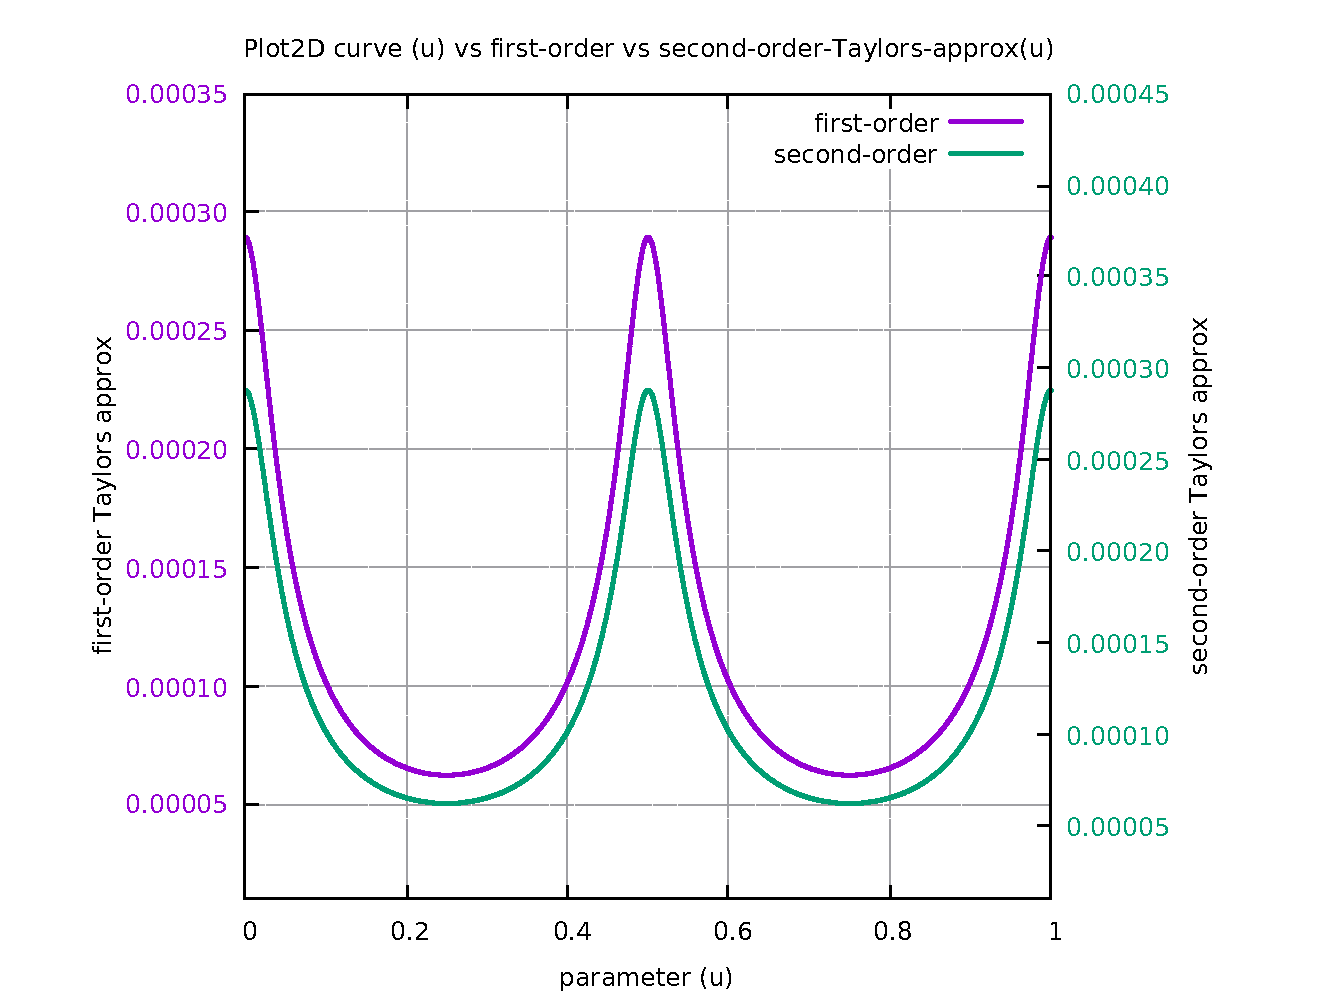
\includegraphics[width=1.00\textwidth]{Chap4/appendix/app-Ellipse/plots/07-img-Ellipse-Separation-First-and-Second-Order-Taylors-Approx.pdf}
\end{figure}


\begin{figure}
	\caption     {Ellipse Separation SAL and SCL}
	\label{08-img-Ellipse-Separation-SAL-and-SCL.pdf}
	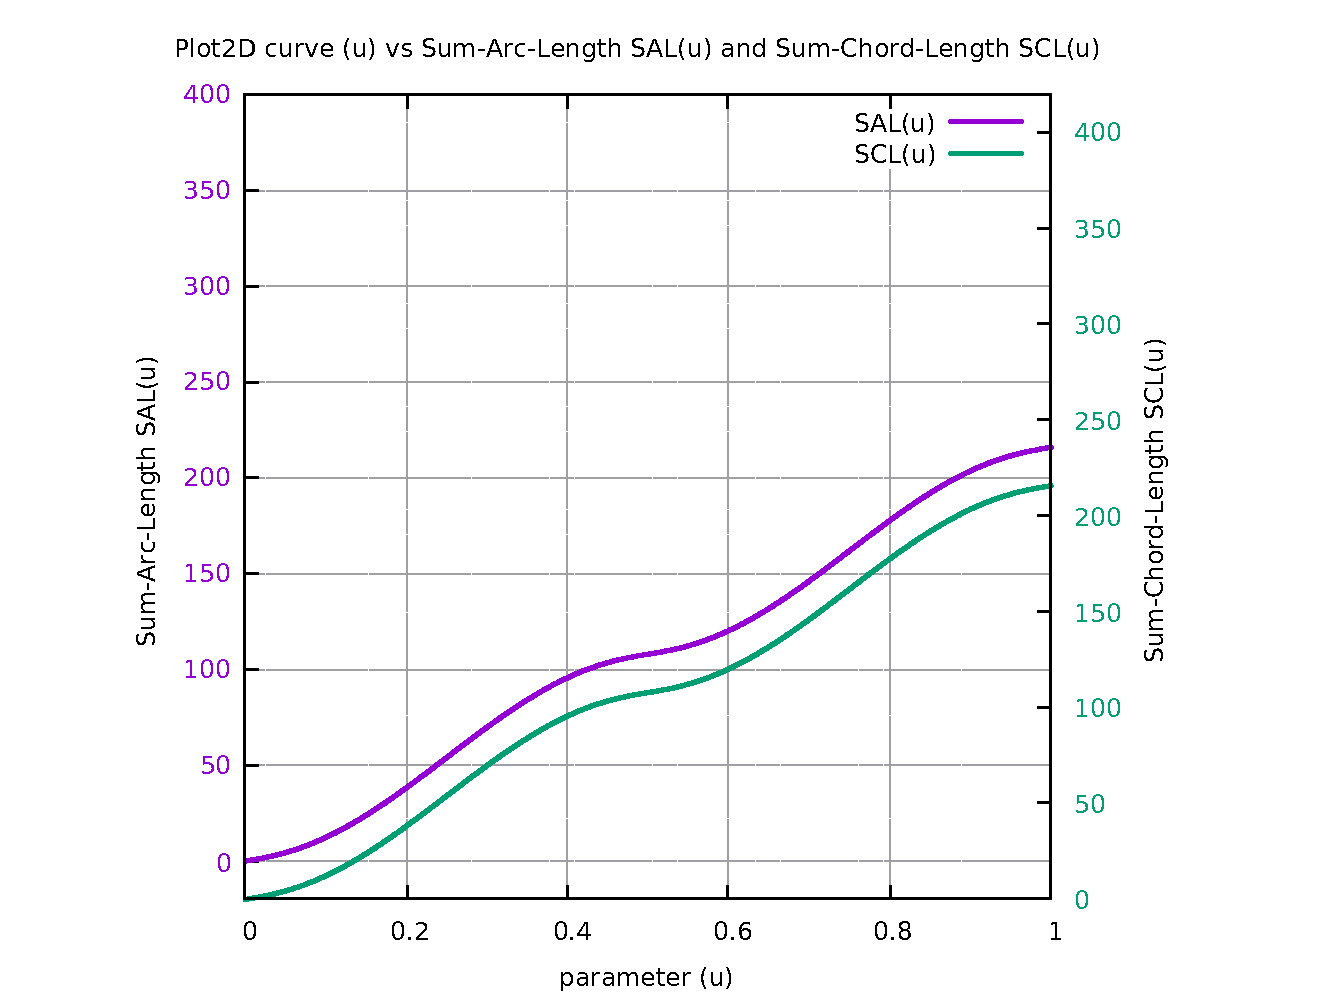
\includegraphics[width=1.00\textwidth]{Chap4/appendix/app-Ellipse/plots/08-img-Ellipse-Separation-SAL-and-SCL.pdf}
\end{figure}

%% ==================================================
\clearpage
\pagebreak

\begin{figure}
	\caption     {Ellipse Chord-error in close view 2 scales}
	\label{09-img-Ellipse-Chord-error-in-close-view-2-scales.pdf}
	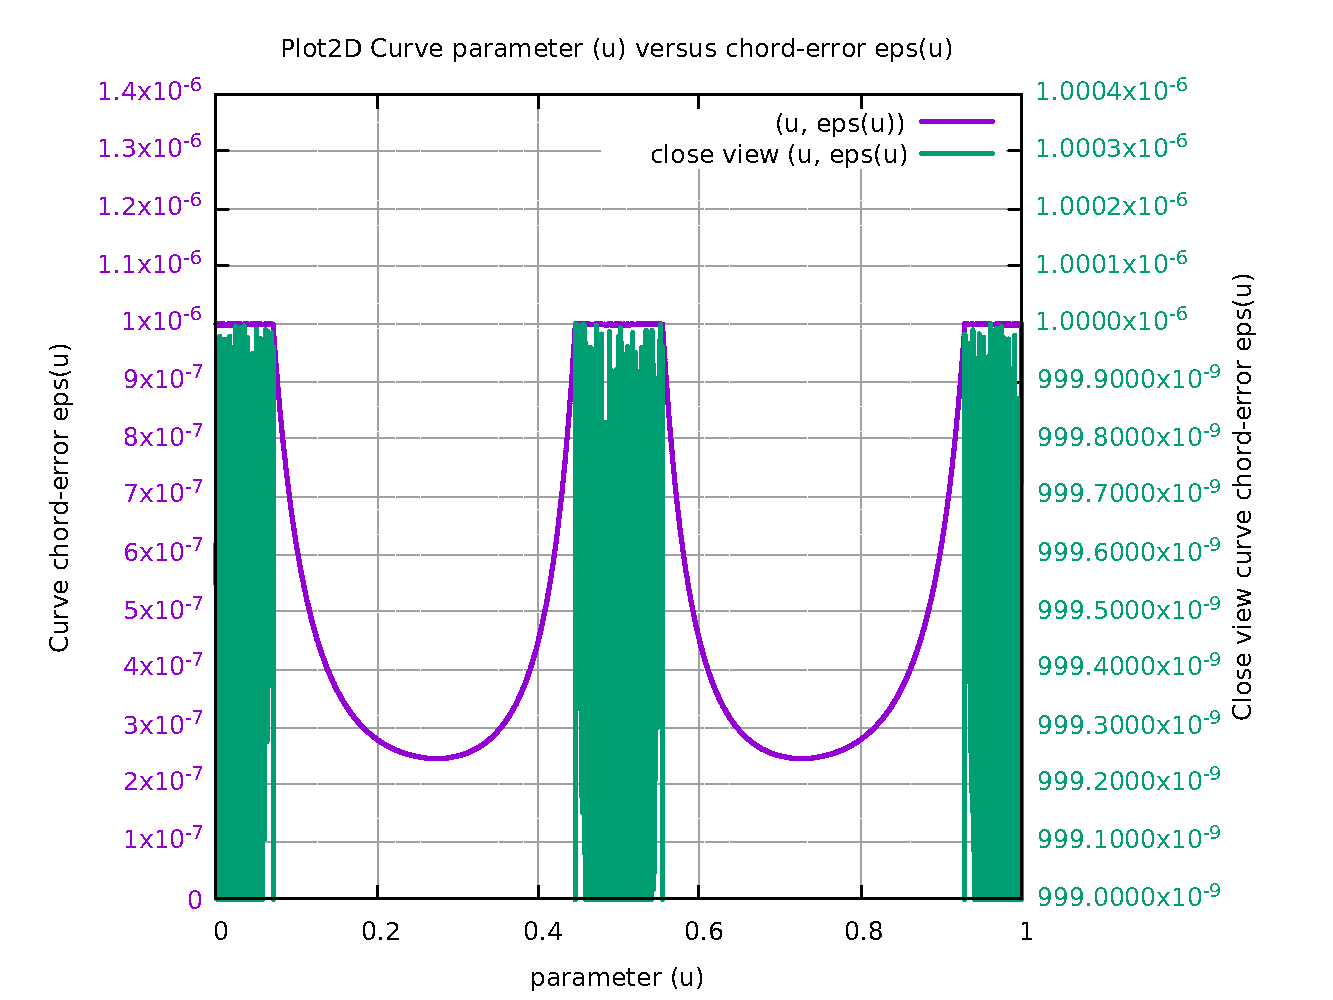
\includegraphics[width=1.00\textwidth]{Chap4/appendix/app-Ellipse/plots/09-img-Ellipse-Chord-error-in-close-view-2-scales.pdf}
\end{figure}

\begin{figure}
	\caption     {Ellipse Four Components Feedrate Limit}
	\label{10-img-Ellipse-Four-Components-Feedrate-Limit.pdf}
	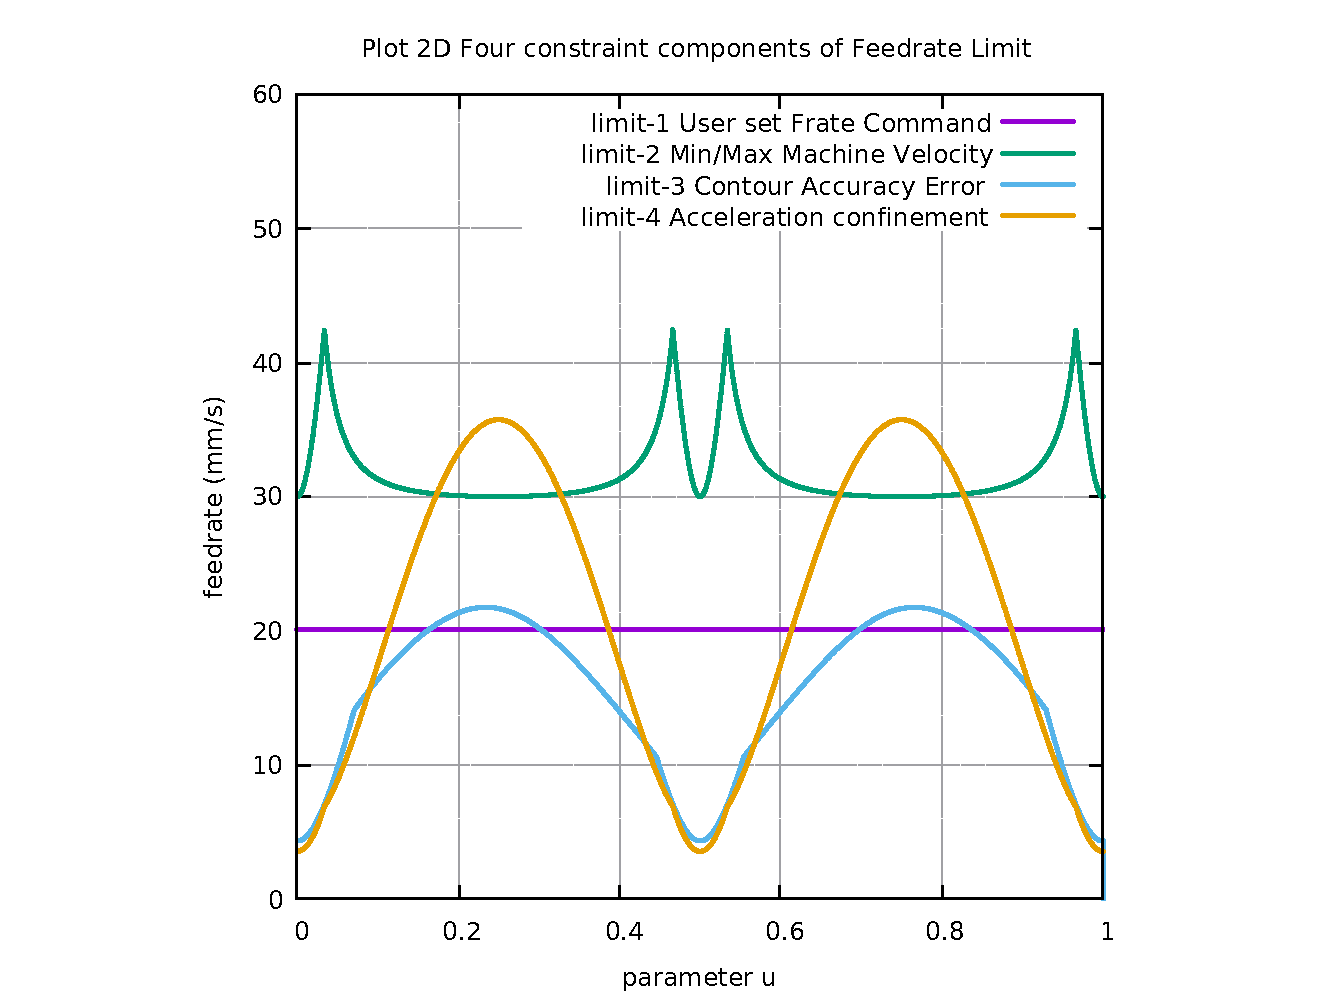
\includegraphics[width=1.00\textwidth]{Chap4/appendix/app-Ellipse/plots/10-img-Ellipse-Four-Components-Feedrate-Limit.pdf}
\end{figure}

%% ==================================================
\clearpage
\pagebreak

\begin{figure}
	\caption     {Ellipse FrateCommand FrateLimit and Curr-Frate}
	\label{11-img-Ellipse-FrateCommand-FrateLimit-and-Curr-Frate.pdf}
	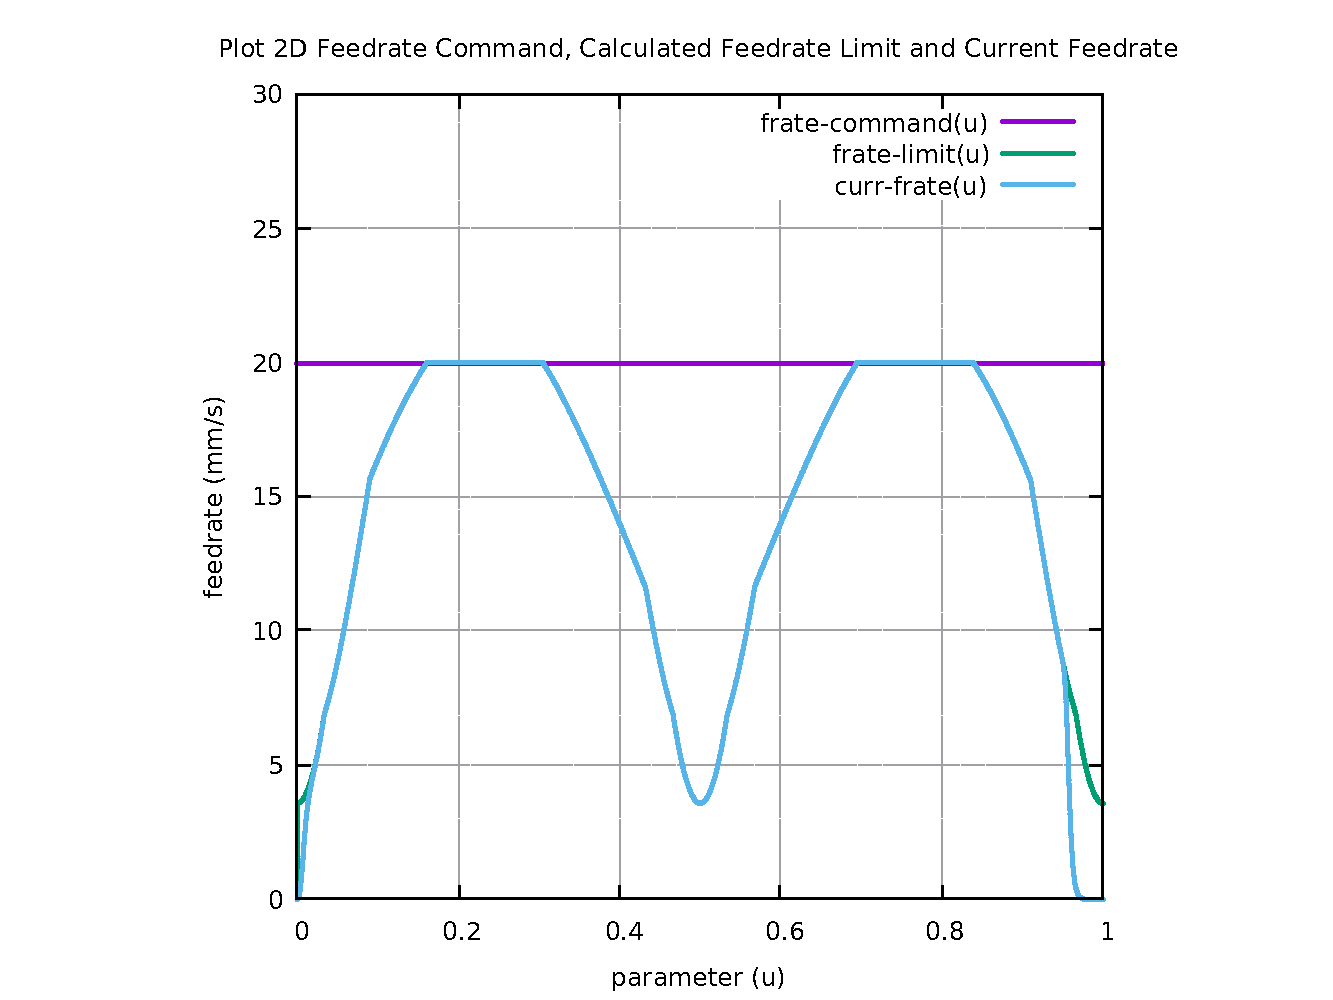
\includegraphics[width=1.00\textwidth]{Chap4/appendix/app-Ellipse/plots/11-img-Ellipse-FrateCommand-FrateLimit-and-Curr-Frate.pdf}
\end{figure}

\begin{figure}
	\caption     {Ellipse FeedRateLimit minus CurrFeedRate}
	\label{12-img-Ellipse-FeedRateLimit-minus-CurrFeedRate.pdf}
	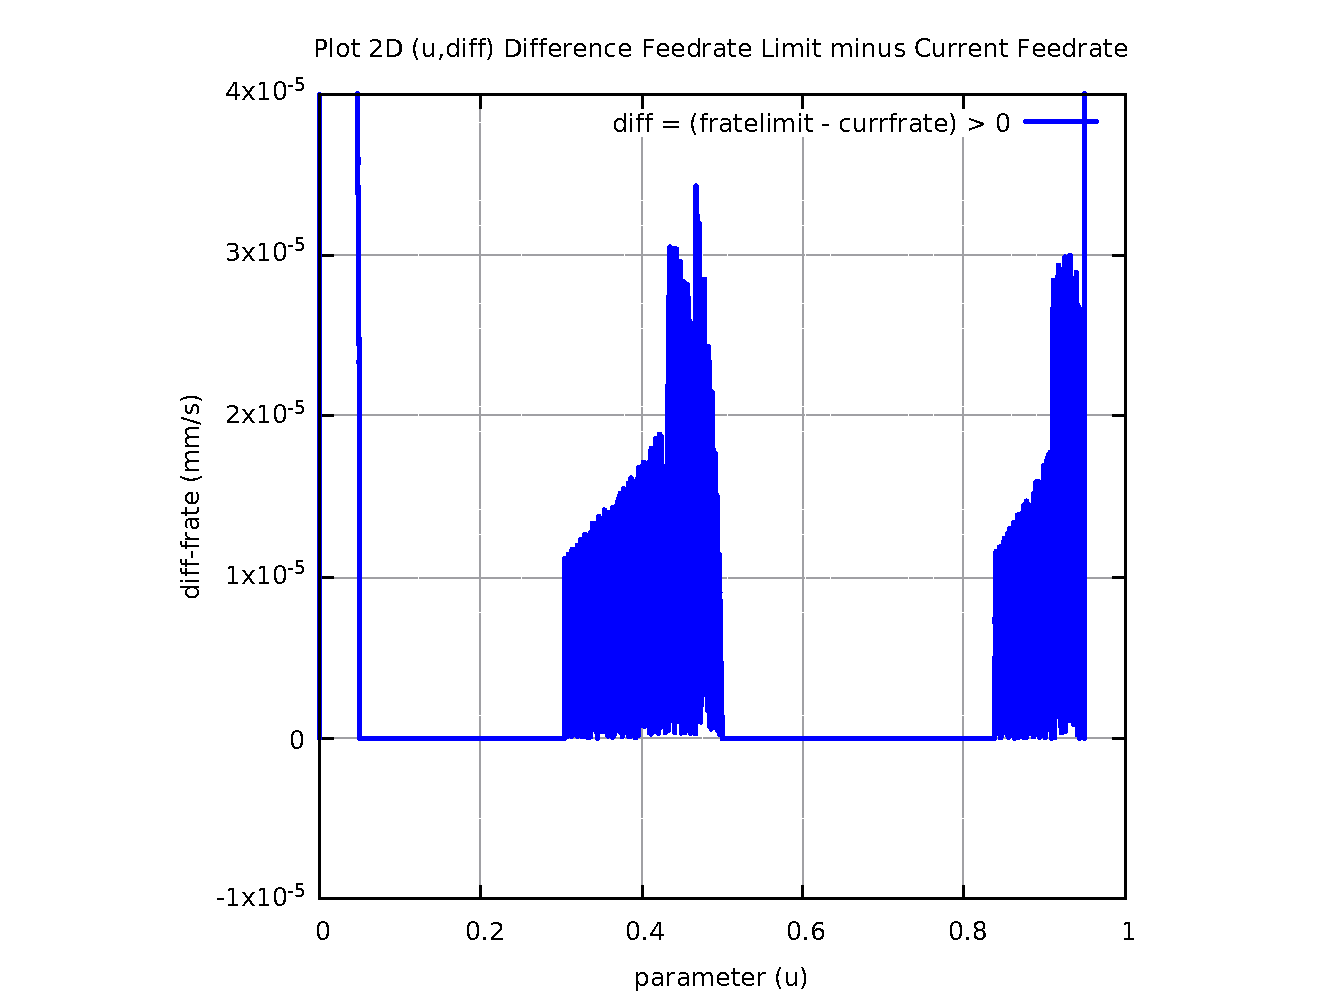
\includegraphics[width=1.00\textwidth]{Chap4/appendix/app-Ellipse/plots/12-img-Ellipse-FeedRateLimit-minus-CurrFeedRate.pdf}
\end{figure}

%% ==================================================
\clearpage
\pagebreak

\begin{figure}
	\caption     {Ellipse FC20-Nominal X and Y Feedrate Profiles}
	\label{13-img-Ellipse-FC20-Nominal-X-and-Y-Feedrate-Profiles.pdf}
	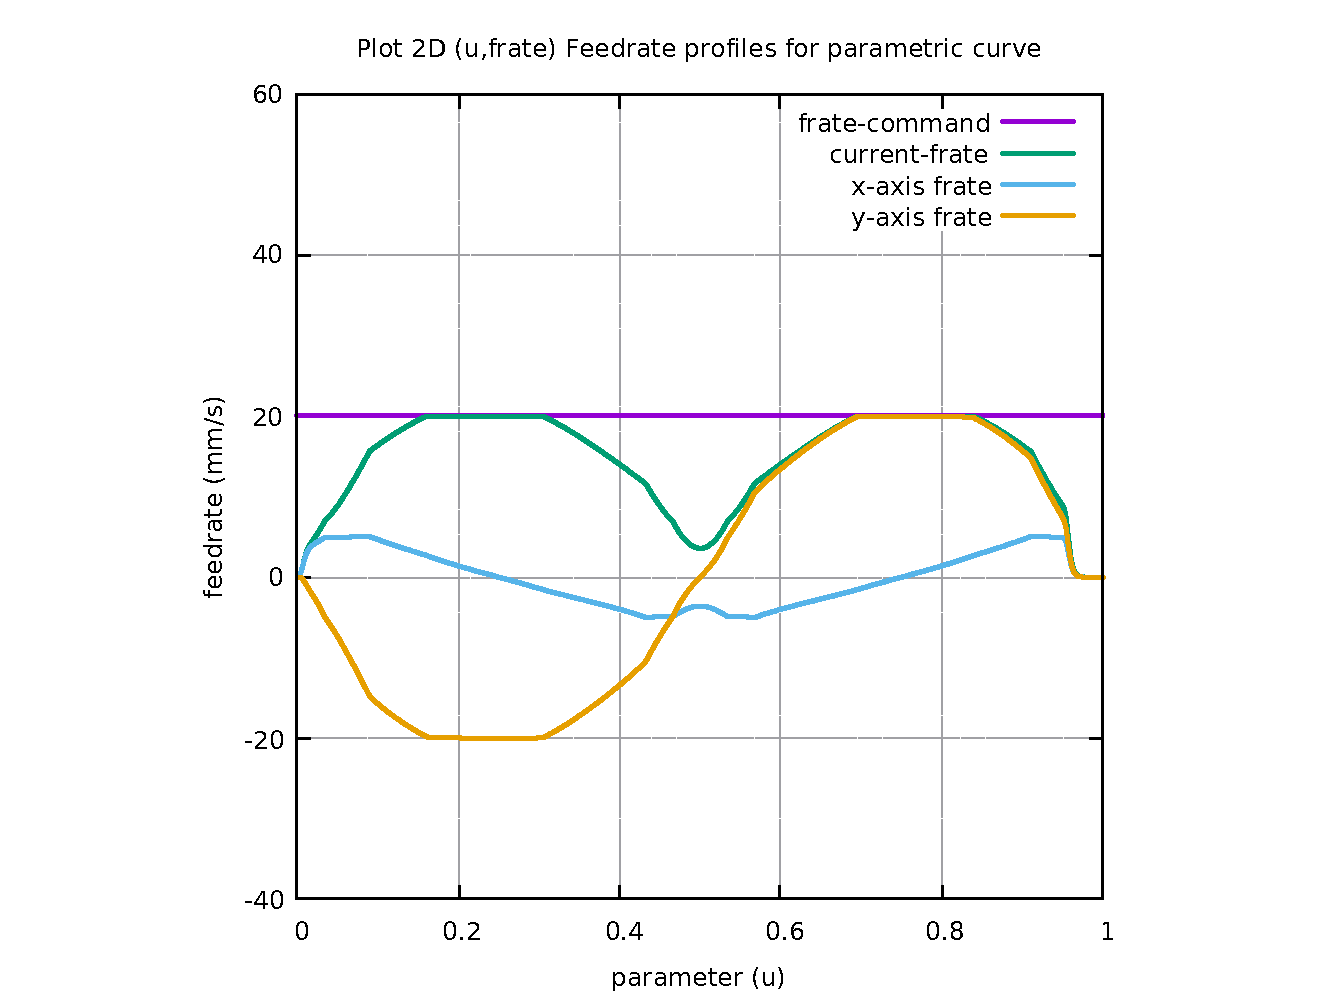
\includegraphics[width=1.00\textwidth]{Chap4/appendix/app-Ellipse/plots/13-img-Ellipse-FC20-Nominal-X-and-Y-Feedrate-Profiles.pdf}
\end{figure}


\begin{figure}
	\caption     {Ellipse FC20 Nominal Tangential Acceleration}
	\label{14-img-Ellipse-FC20-Nominal-Tangential-Acceleration.pdf}
	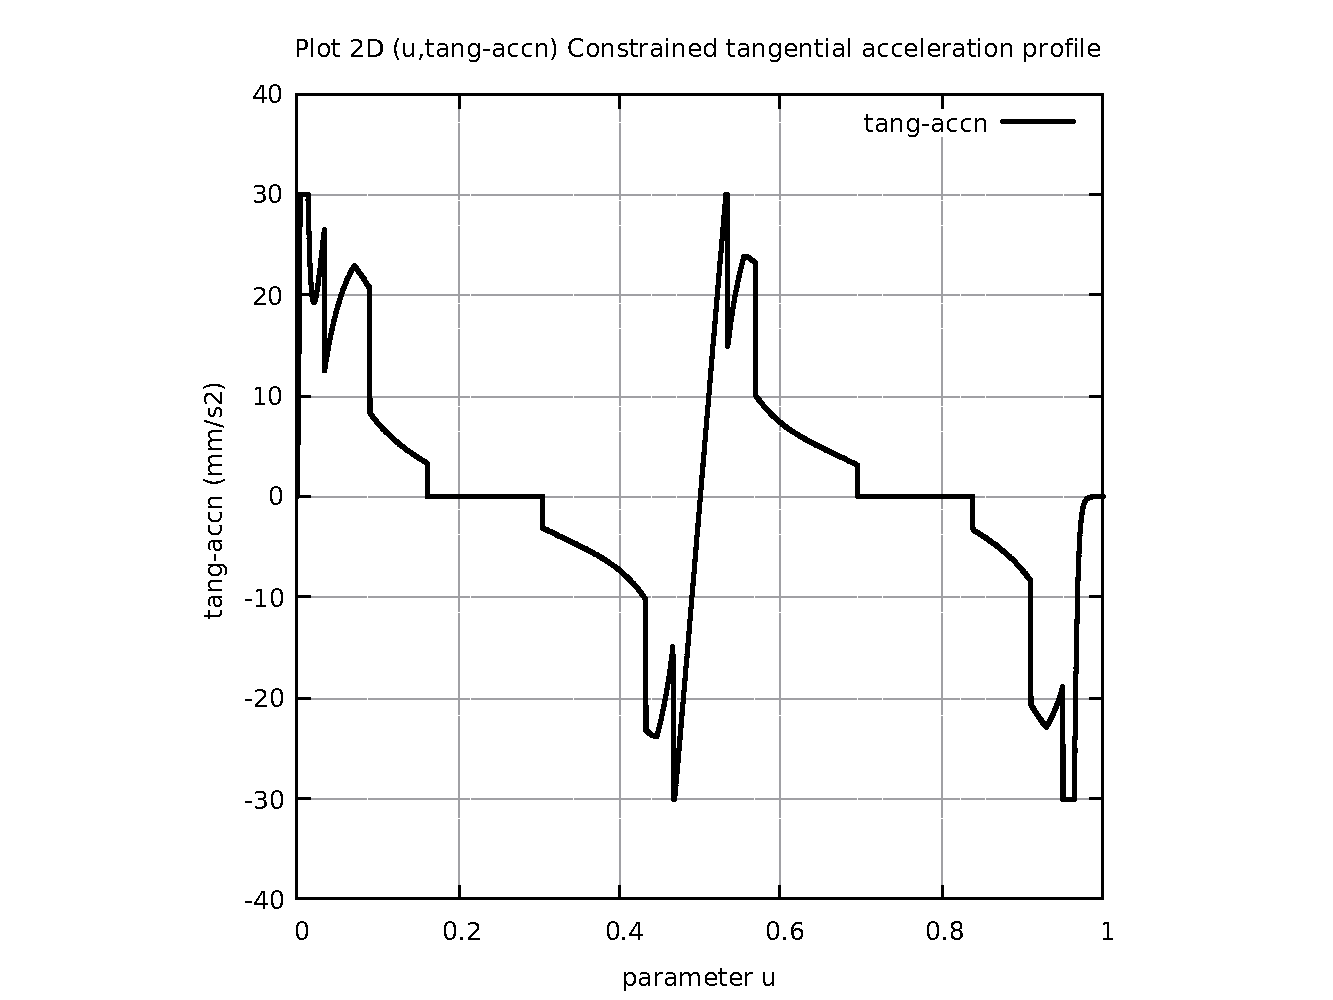
\includegraphics[width=1.00\textwidth]{Chap4/appendix/app-Ellipse/plots/14-img-Ellipse-FC20-Nominal-Tangential-Acceleration.pdf}
\end{figure}

%% ==================================================
\clearpage
\pagebreak

\begin{figure}
	\caption     {Ellipse FC20 Nominal Rising S-Curve Profile}
	\label{15-img-Ellipse-FC20-Nominal-Rising-S-Curve-Profile.pdf}
	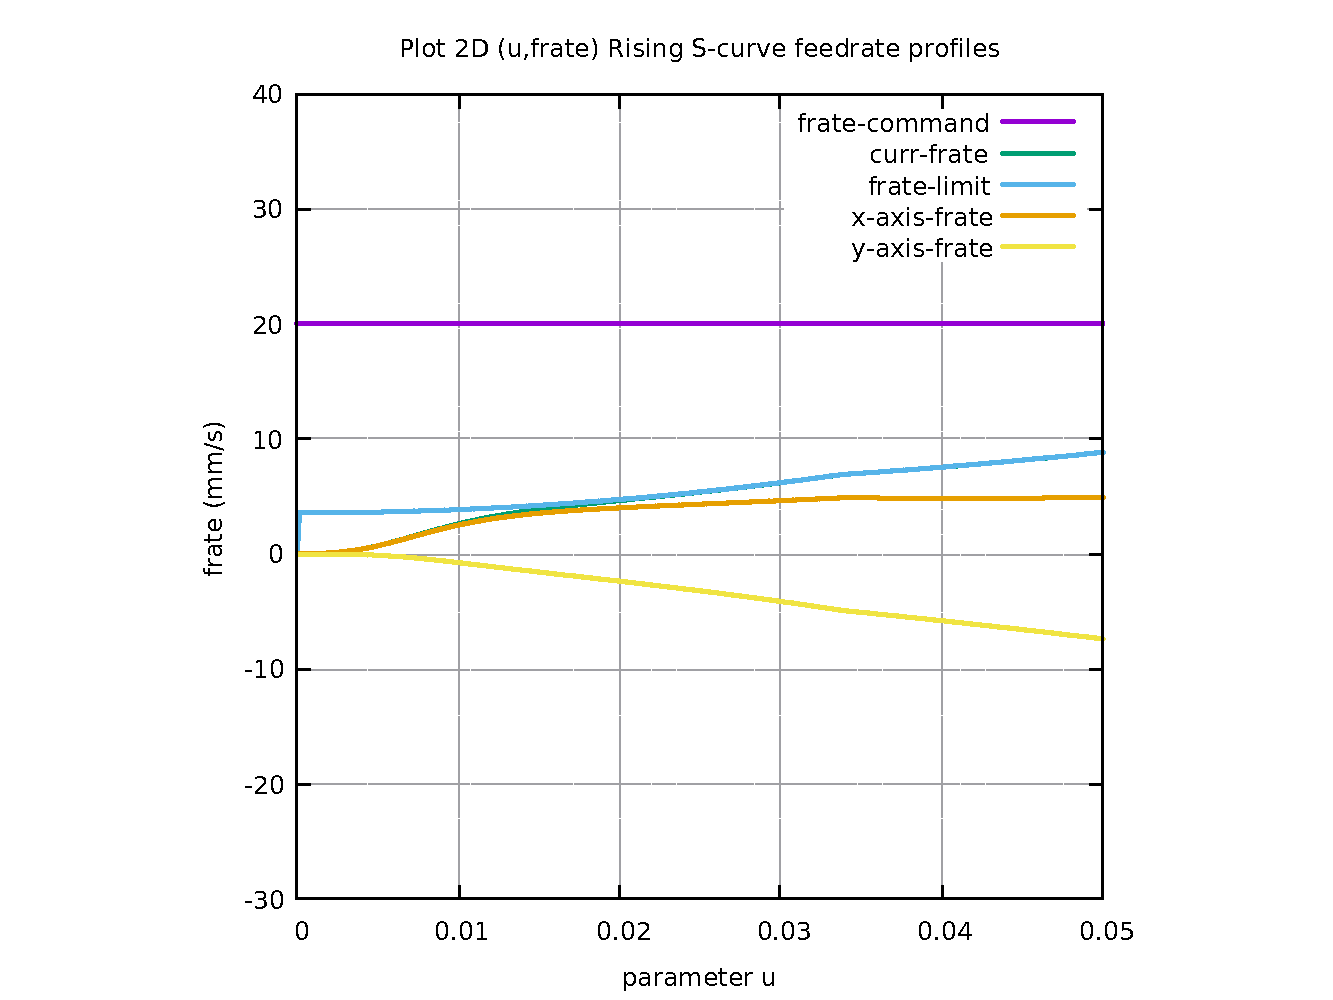
\includegraphics[width=1.00\textwidth]{Chap4/appendix/app-Ellipse/plots/15-img-Ellipse-FC20-Nominal-Rising-S-Curve-Profile.pdf}
\end{figure}


\begin{figure}
	\caption     {Ellipse FC20 Nominal Falling S-Curve Profile}
	\label{16-img-Ellipse-FC20-Nominal-Falling-S-Curve-Profile.pdf}
	%%	\centering
	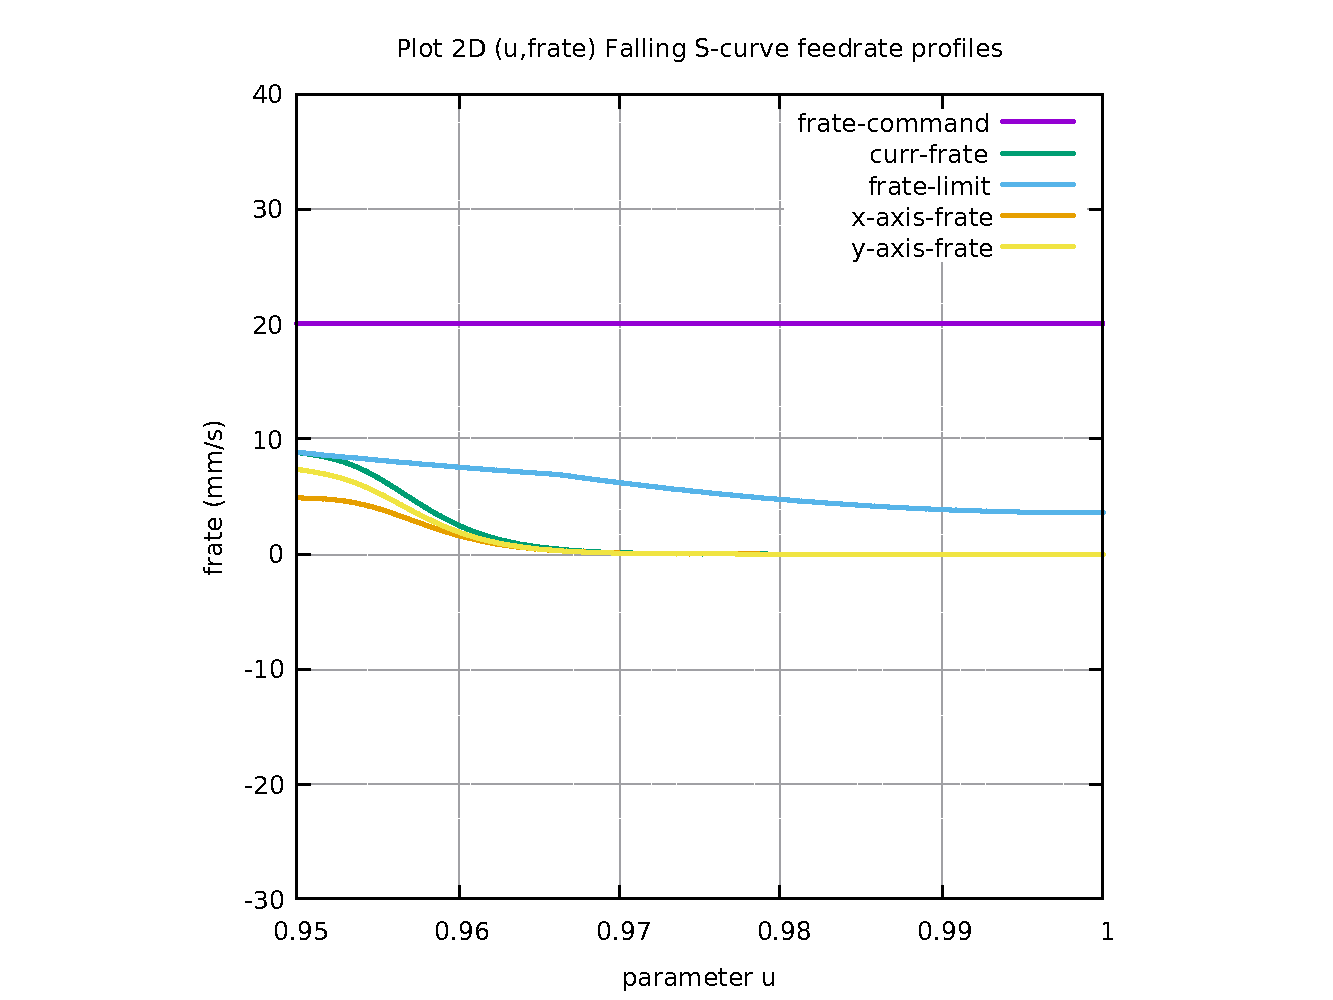
\includegraphics[width=1.00\textwidth]{Chap4/appendix/app-Ellipse/plots/16-img-Ellipse-FC20-Nominal-Falling-S-Curve-Profile.pdf}
\end{figure}

%% ==================================================
\clearpage
\pagebreak

\begin{figure}
	\caption     {Ellipse FC10 Colored Feedrate Profile data ngcode}
	\label{17-img-Ellipse-FC10-Colored-Feedrate-Profile-data_ngcode.png}
	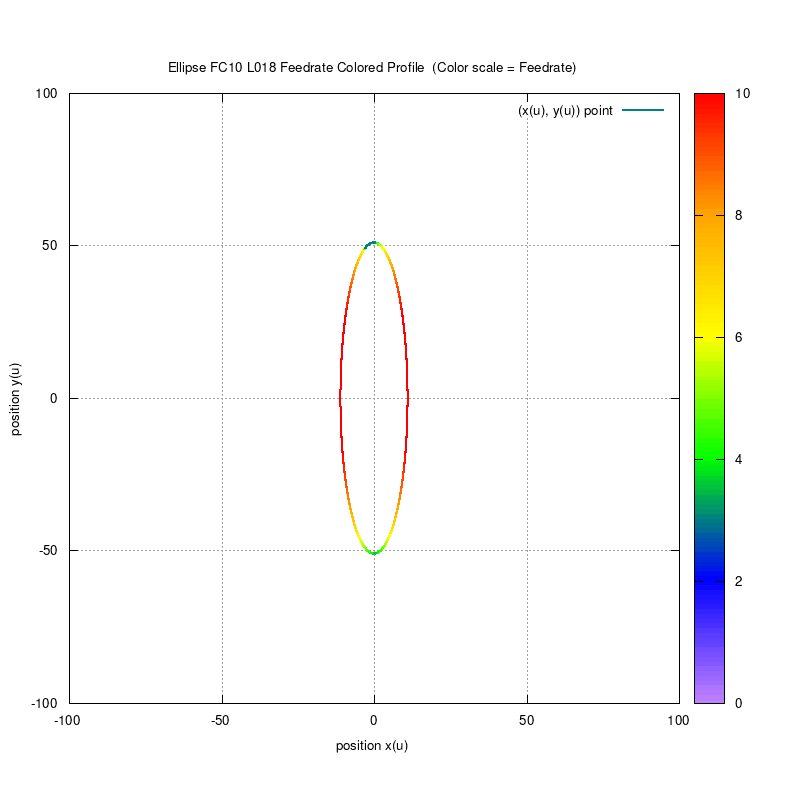
\includegraphics[width=0.75\textwidth]{Chap4/appendix/app-Ellipse/plots/17-img-Ellipse-FC10-Colored-Feedrate-Profile-data_ngcode.png}
\end{figure}


\begin{figure}
	\caption     {Ellipse FC20 Colored Feedrate Profile data ngcode}
	\label{18-img-Ellipse-FC20-Colored-Feedrate-Profile-data_ngcode.png}
	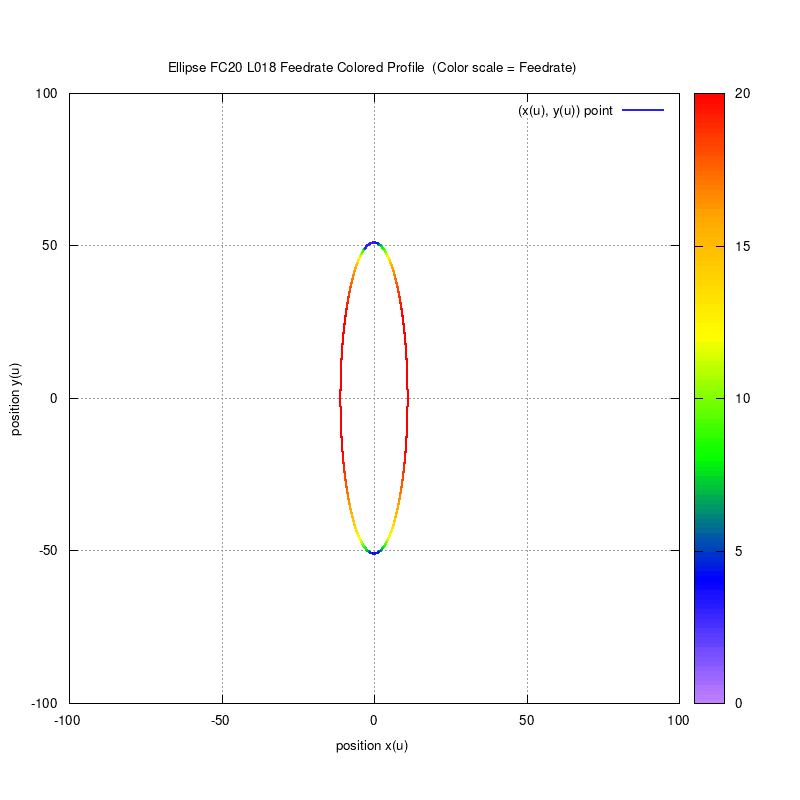
\includegraphics[width=0.75\textwidth]{Chap4/appendix/app-Ellipse/plots/18-img-Ellipse-FC20-Colored-Feedrate-Profile-data_ngcode.png}
\end{figure}

%% ==================================================
\clearpage
\pagebreak

\begin{figure}
	\caption     {Ellipse FC30 Colored Feedrate Profile data ngcode}
	\label{19-img-Ellipse-FC30-Colored-Feedrate-Profile-data_ngcode.png}
	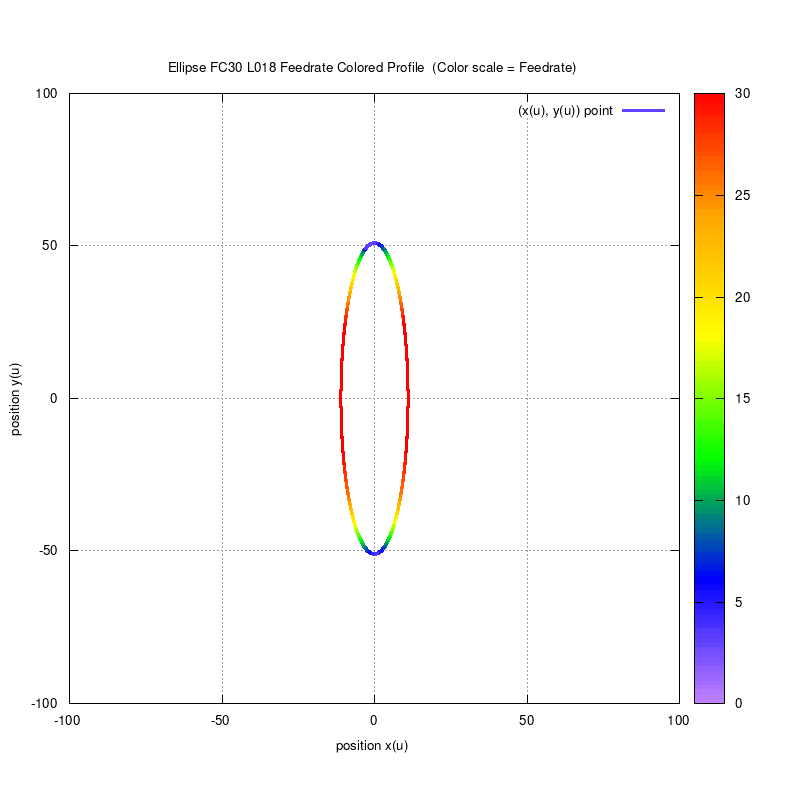
\includegraphics[width=0.75\textwidth]{Chap4/appendix/app-Ellipse/plots/19-img-Ellipse-FC30-Colored-Feedrate-Profile-data_ngcode.png}
\end{figure}


\begin{figure}
	\caption     {Ellipse FC40 Colored Feedrate Profile data ngcode}
	\label{20-img-Ellipse-FC40-Colored-Feedrate-Profile-data_ngcode.png}
	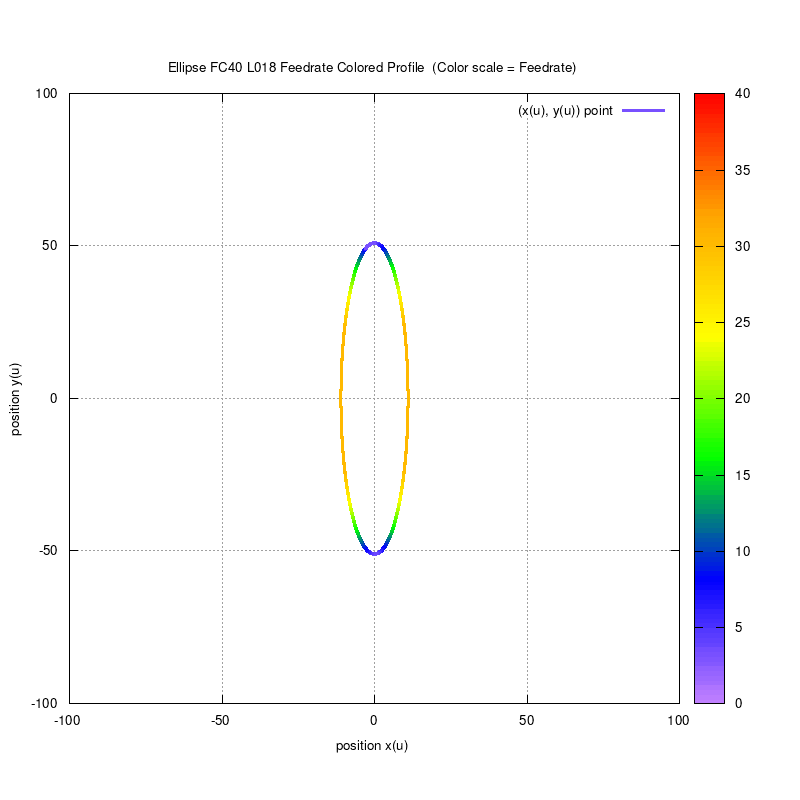
\includegraphics[width=0.75\textwidth]{Chap4/appendix/app-Ellipse/plots/20-img-Ellipse-FC40-Colored-Feedrate-Profile-data_ngcode.png}
\end{figure}

%% ==================================================
\clearpage
\pagebreak

\begin{figure}
	\caption     {Ellipse FC10 Tangential Acceleration}
	\label{21-img-Ellipse-FC10-Tangential-Acceleration.pdf}
	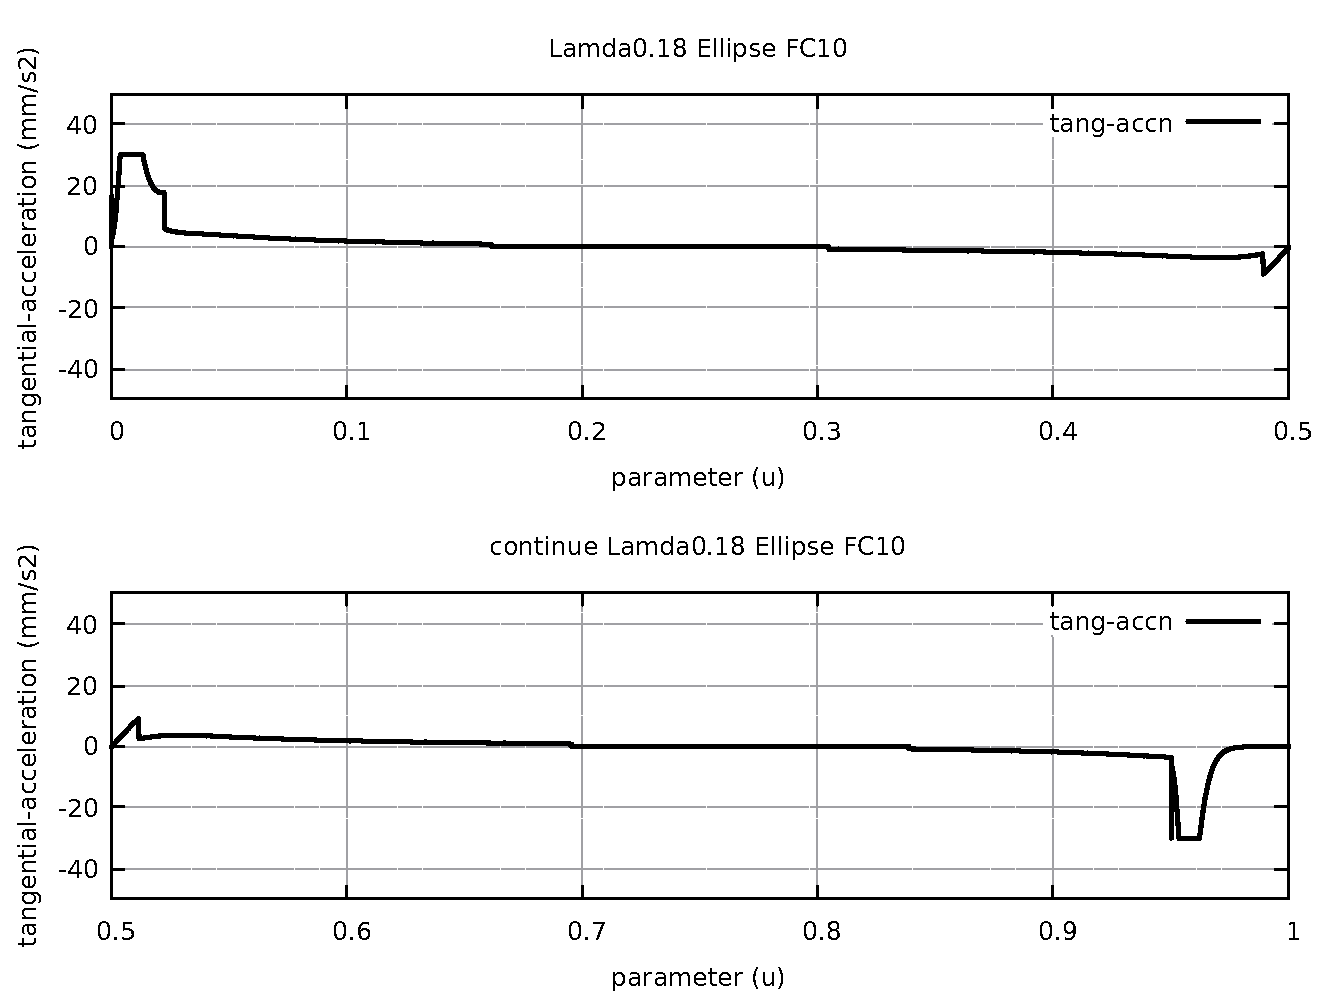
\includegraphics[width=1.00\textwidth]{Chap4/appendix/app-Ellipse/plots/21-img-Ellipse-FC10-Tangential-Acceleration.pdf}
\end{figure}


\begin{figure}
	\caption     {Ellipse FC20 Tangential Acceleration}
	\label{22-img-Ellipse-FC20-Tangential-Acceleration.pdf}
	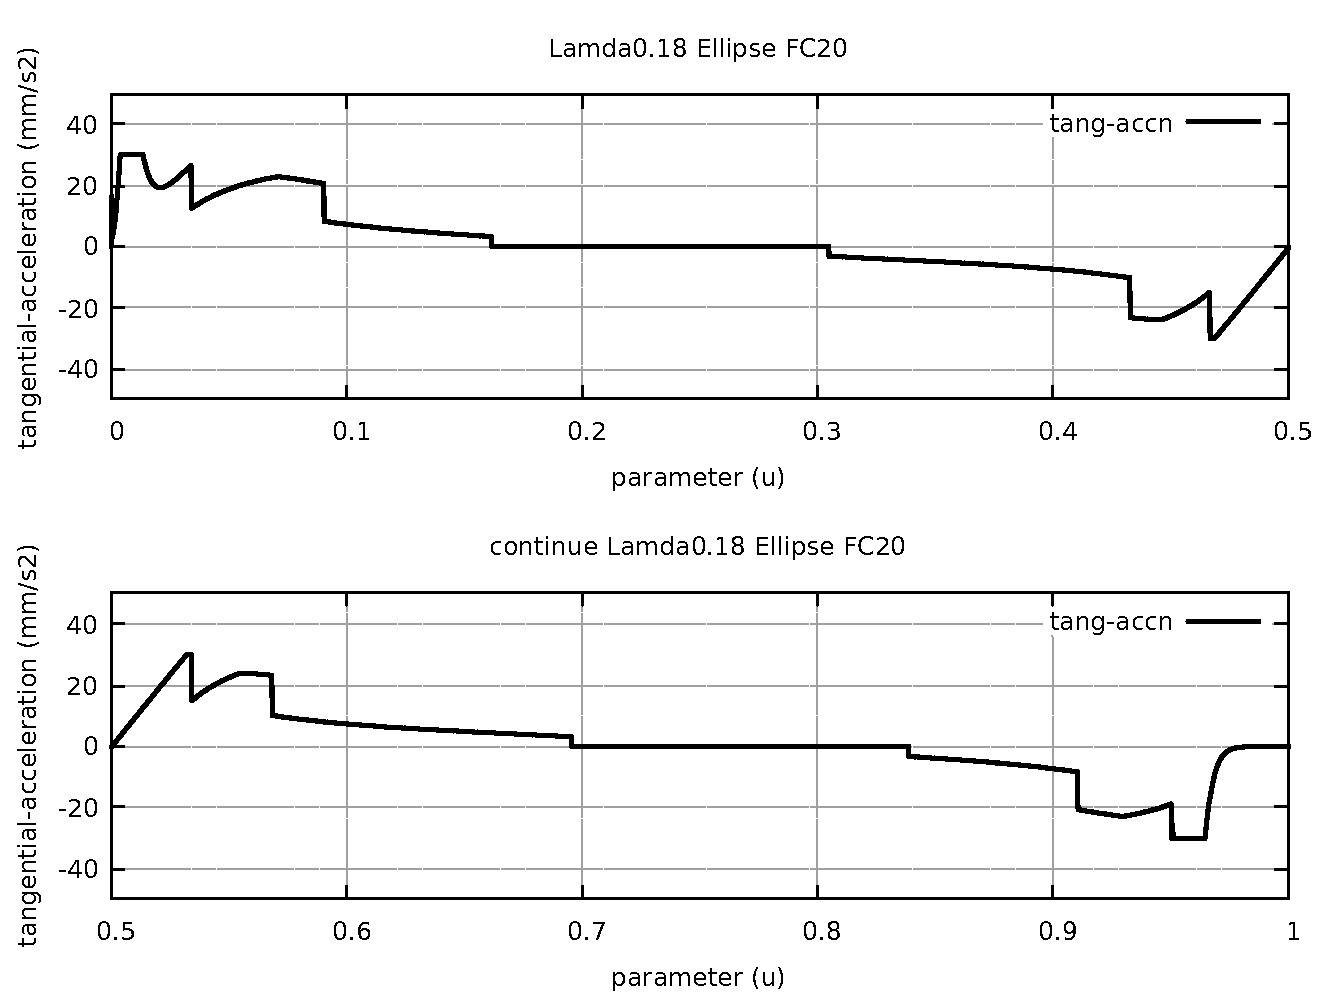
\includegraphics[width=1.00\textwidth]{Chap4/appendix/app-Ellipse/plots/22-img-Ellipse-FC20-Tangential-Acceleration.pdf}
\end{figure}

%% ==================================================
\clearpage
\pagebreak

\begin{figure}
	\caption     {Ellipse FC30 Tangential Acceleration}
	\label{23-img-Ellipse-FC30-Tangential-Acceleration.pdf}
	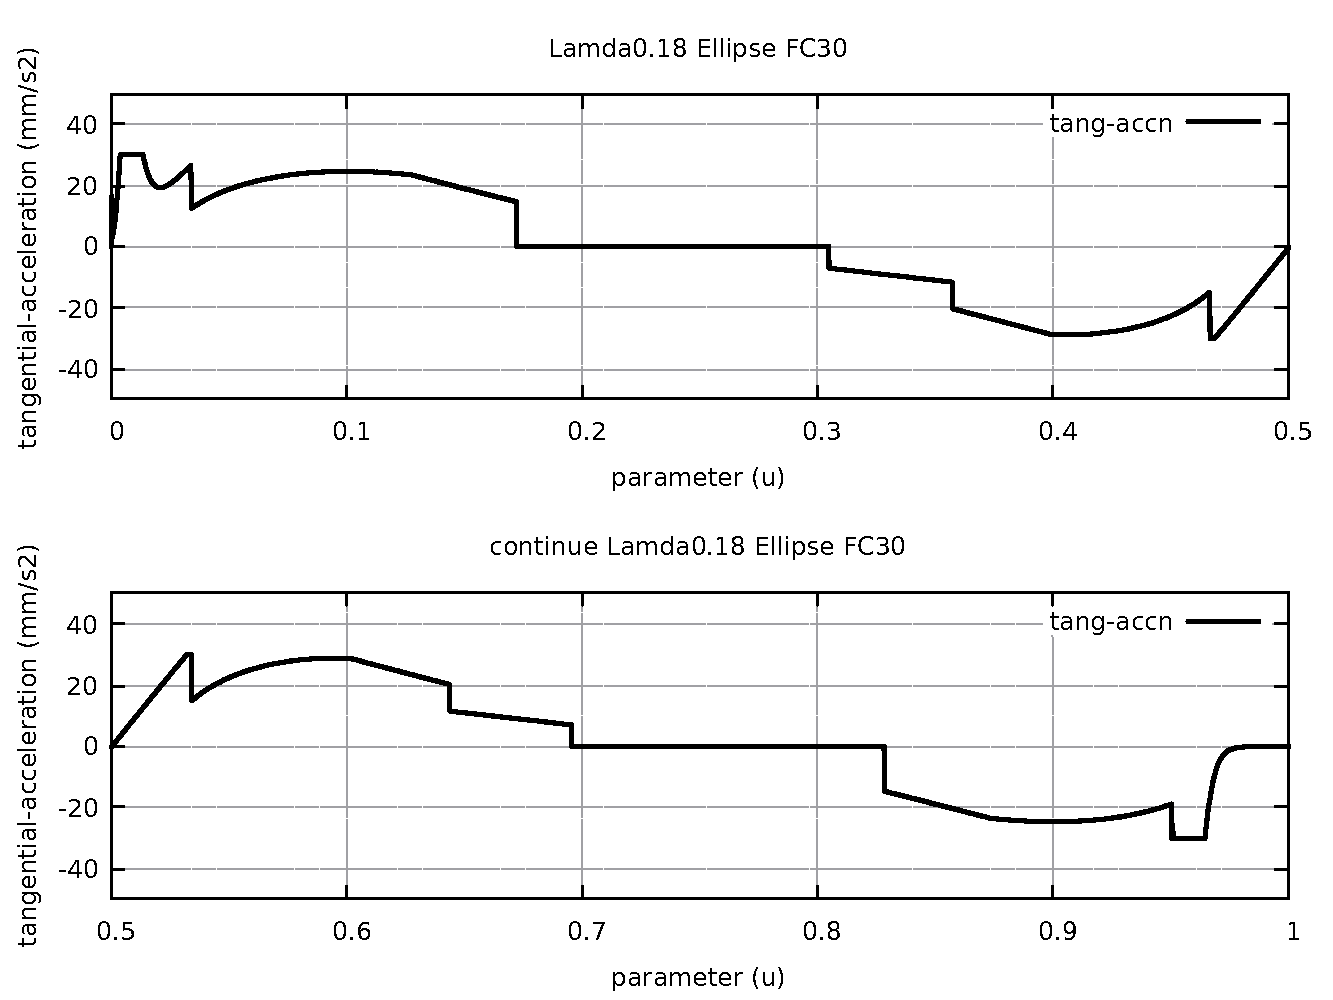
\includegraphics[width=1.00\textwidth]{Chap4/appendix/app-Ellipse/plots/23-img-Ellipse-FC30-Tangential-Acceleration.pdf}
\end{figure}


\begin{figure}
	\caption     {Ellipse FC40 Tangential Acceleration}
	\label{24-img-Ellipse-FC40-Tangential-Acceleration.pdf}
	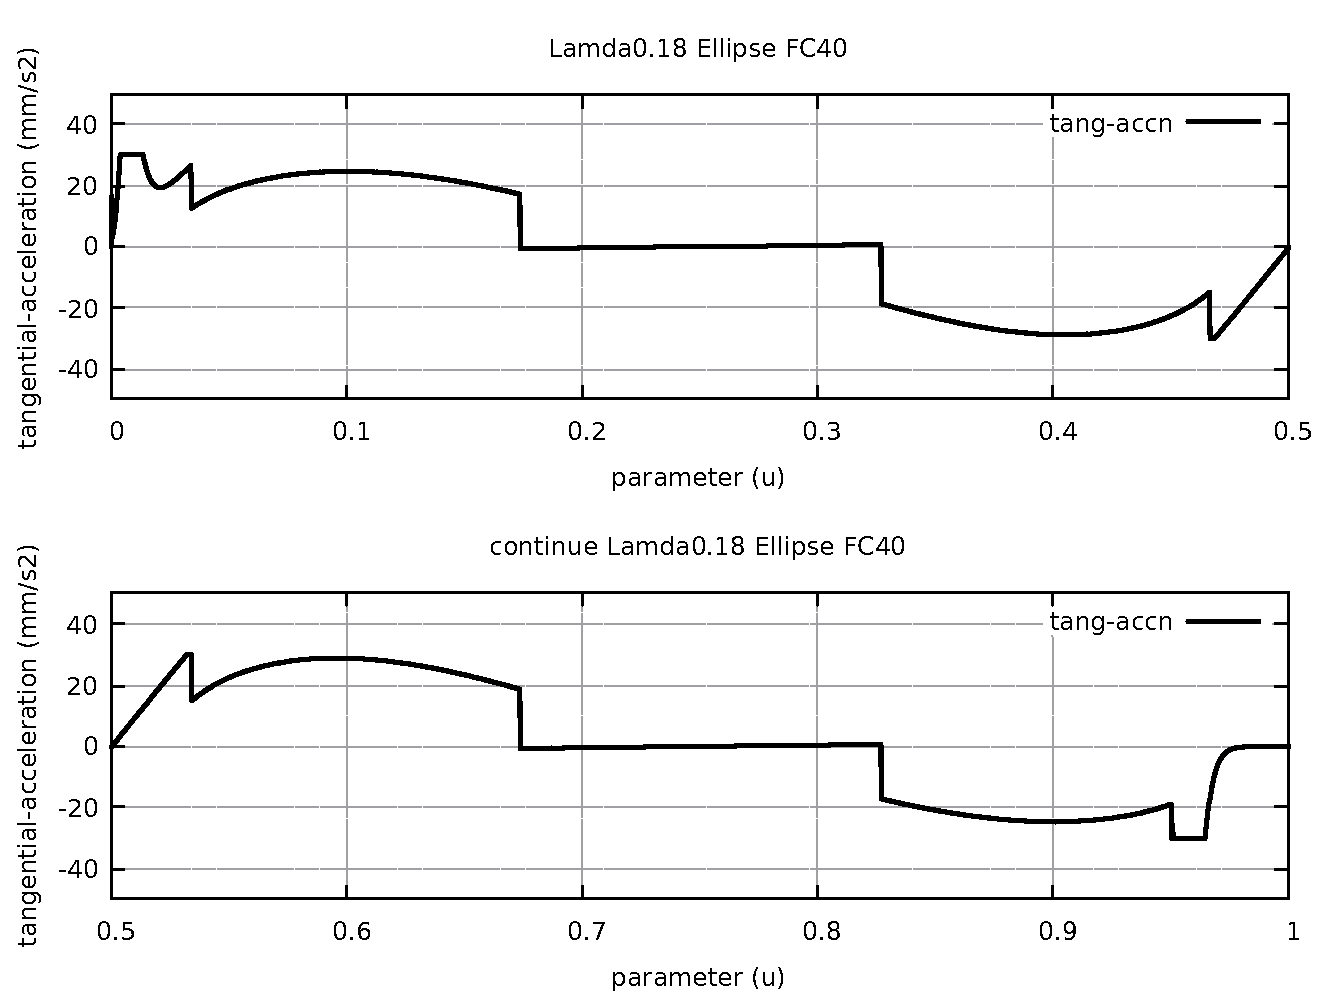
\includegraphics[width=1.00\textwidth]{Chap4/appendix/app-Ellipse/plots/24-img-Ellipse-FC40-Tangential-Acceleration.pdf}
\end{figure}

%% ==================================================
\clearpage
\pagebreak

\begin{figure}
	\caption     {Ellipse FC20 Nominal Separation NAL and NCL}
	\label{25-img-Ellipse-FC20-Nominal-Separation-NAL-and-NCL.pdf}
	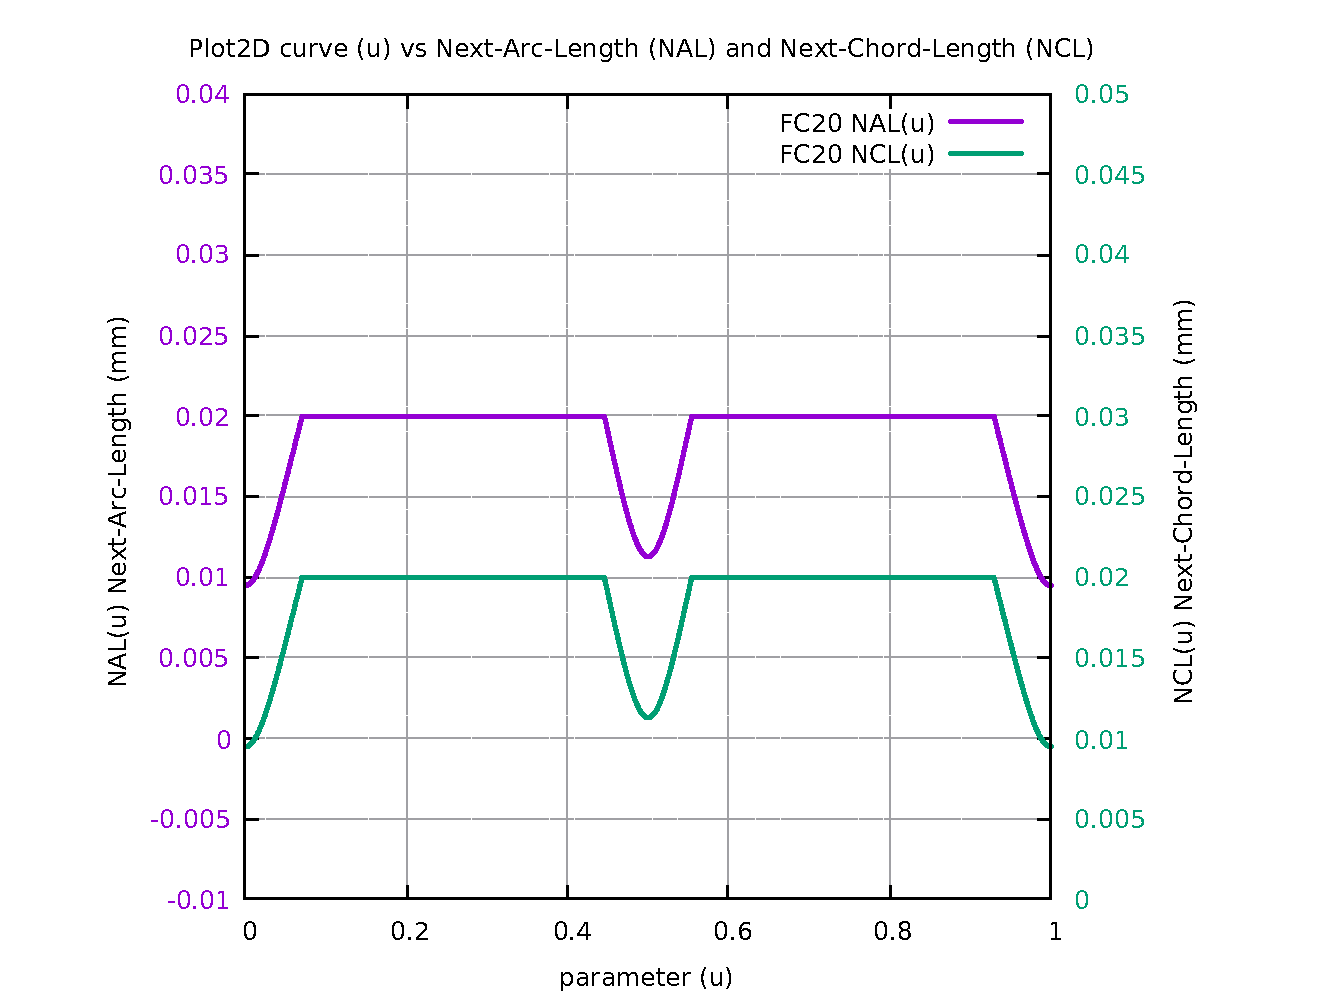
\includegraphics[width=1.00\textwidth]{Chap4/appendix/app-Ellipse/plots/25-img-Ellipse-FC20-Nominal-Separation-NAL-and-NCL.pdf}
\end{figure}


\begin{figure}
	\caption     {Ellipse Difference SAL minus SCL for FC10 FC20 FC30 FC40}
	\label{26-img-Ellipse-Difference-SAL-minus-SCL-for-FC10-FC20-FC30-FC40.pdf}
	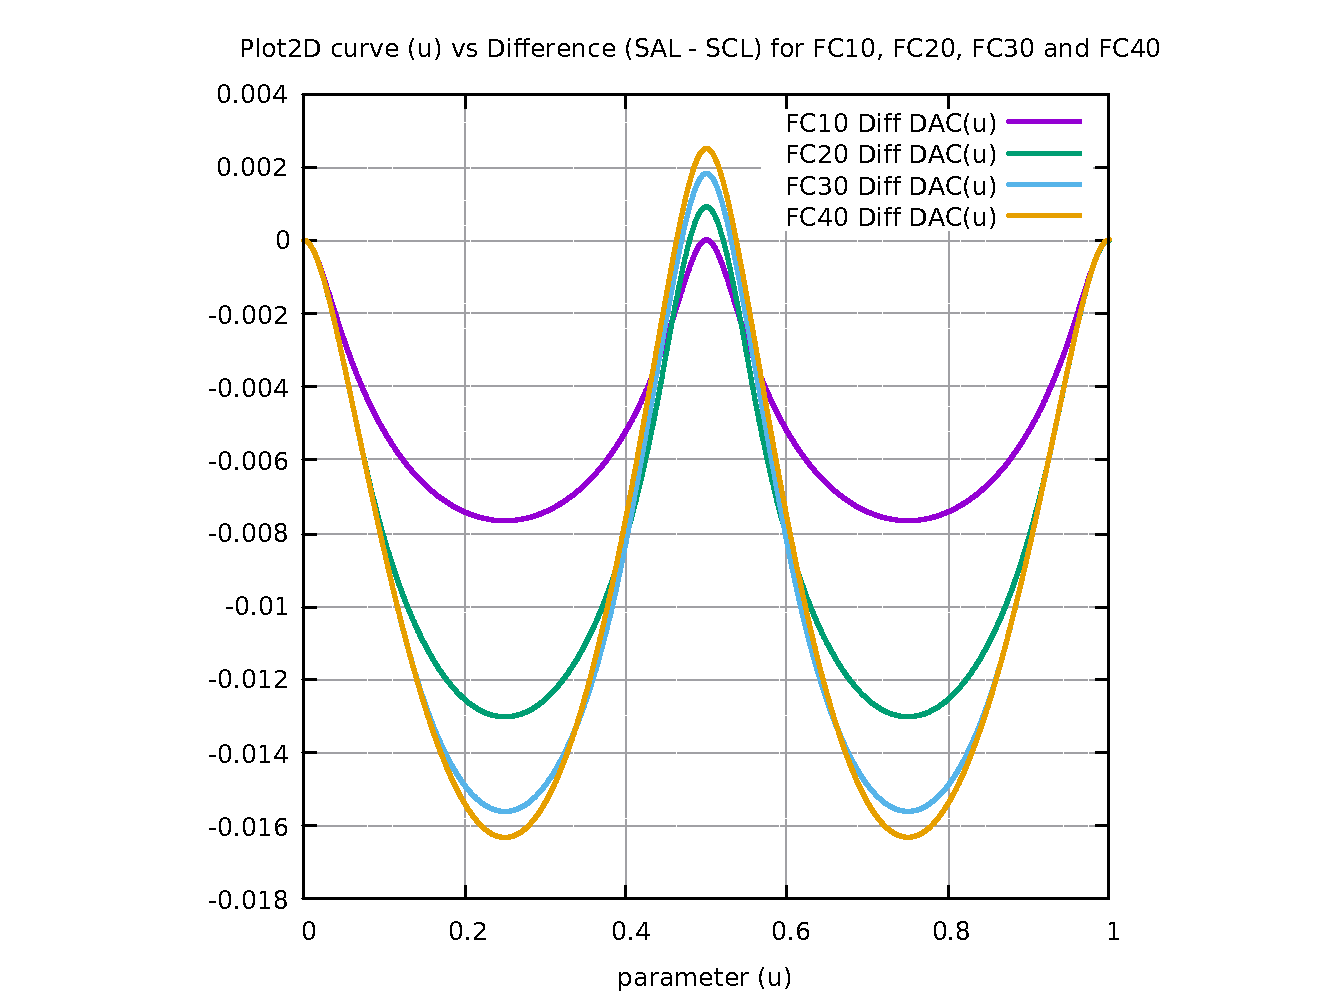
\includegraphics[width=1.00\textwidth]{Chap4/appendix/app-Ellipse/plots/26-img-Ellipse-Difference-SAL-minus-SCL-for-FC10-FC20-FC30-FC40.pdf}
\end{figure}


%% ==================================================
\clearpage
\pagebreak

\begin{figure}
	\caption     {Ellipse FC10 FrateCmd CurrFrate X-Frate Y-Frate}
	\label{27-img-Ellipse-FC10-FrateCmd-CurrFrate-X-Frate-Y-Frate.pdf}
	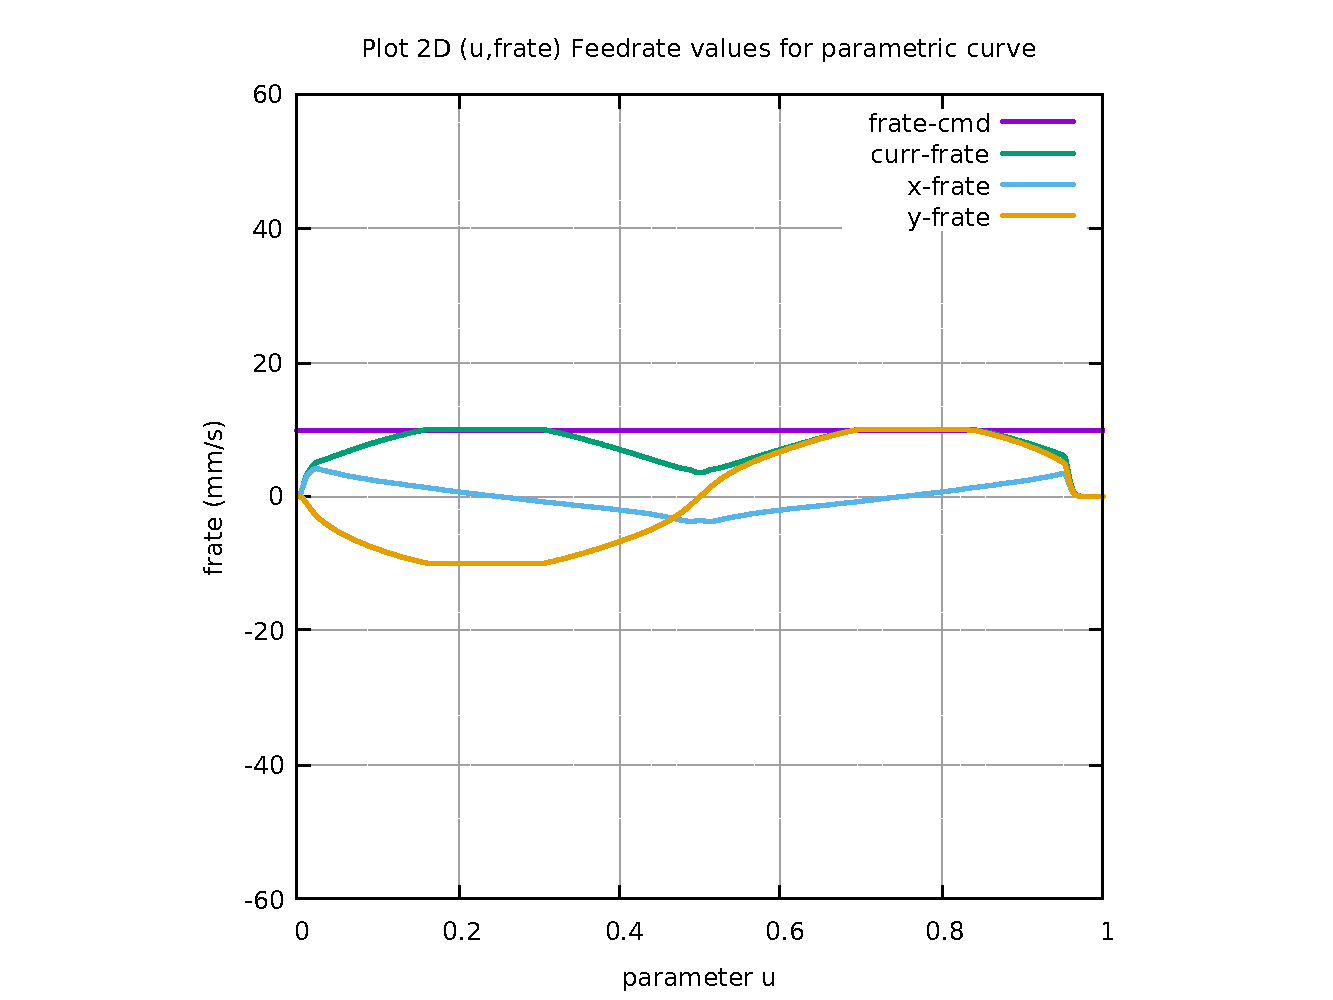
\includegraphics[width=1.00\textwidth]{Chap4/appendix/app-Ellipse/plots/27-img-Ellipse-FC10-FrateCmd-CurrFrate-X-Frate-Y-Frate.pdf}
\end{figure}


\begin{figure}
	\caption     {Ellipse FC20 FrateCmd CurrFrate X-Frate Y-Frate}
	\label{28-img-Ellipse-FC20-FrateCmd-CurrFrate-X-Frate-Y-Frate.pdf}
	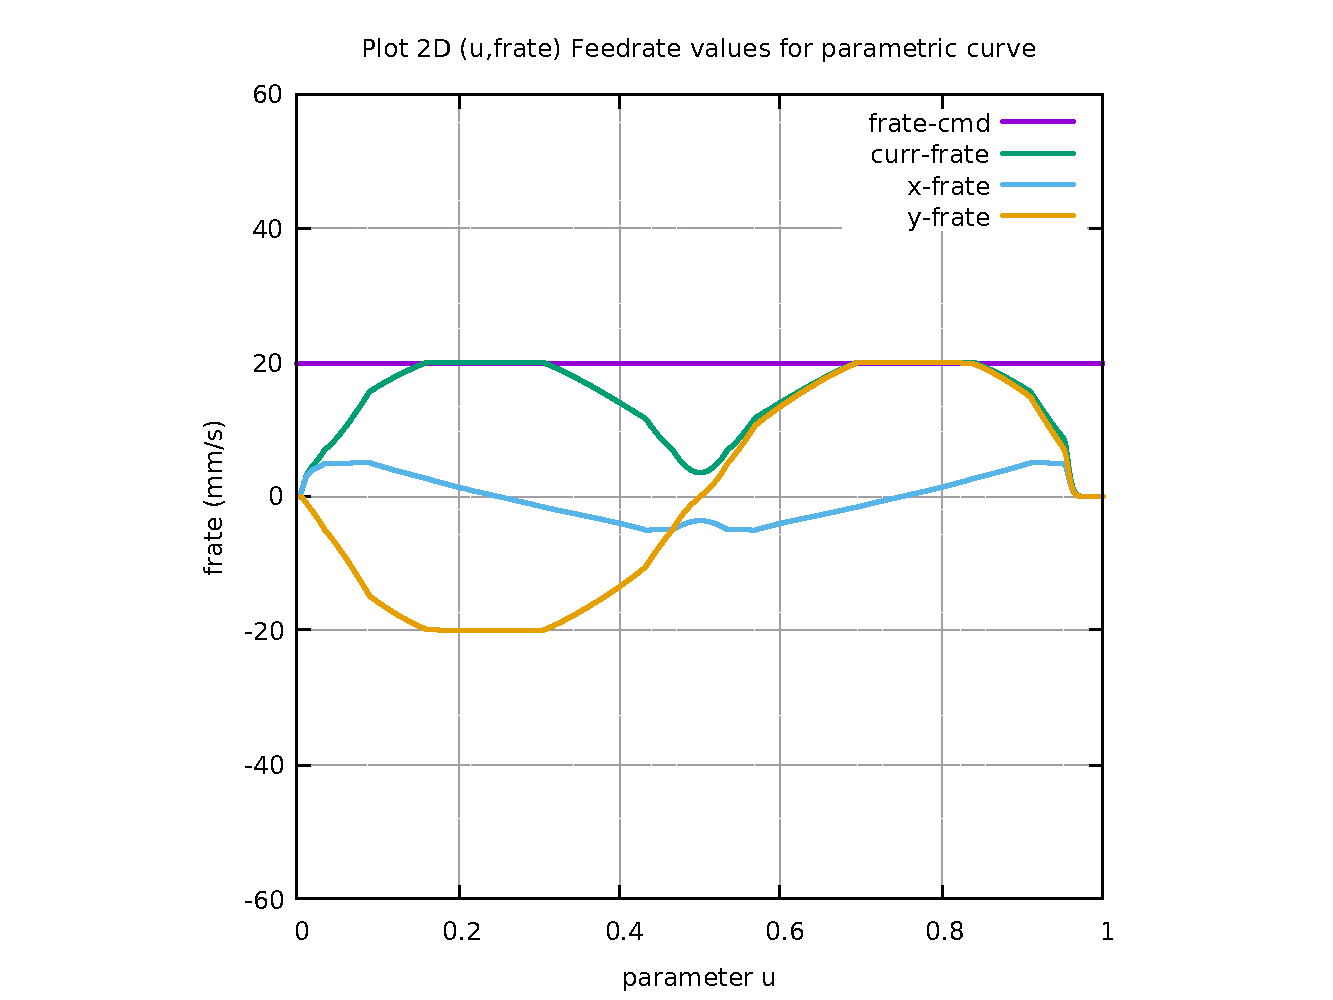
\includegraphics[width=1.00\textwidth]{Chap4/appendix/app-Ellipse/plots/28-img-Ellipse-FC20-FrateCmd-CurrFrate-X-Frate-Y-Frate.pdf}
\end{figure}


%% ==================================================
\clearpage
\pagebreak

\begin{figure}
	\caption     {Ellipse FC30 FrateCmd CurrFrate X-Frate Y-Frate}
	\label{29-img-Ellipse-FC30-FrateCmd-CurrFrate-X-Frate-Y-Frate.pdf}
	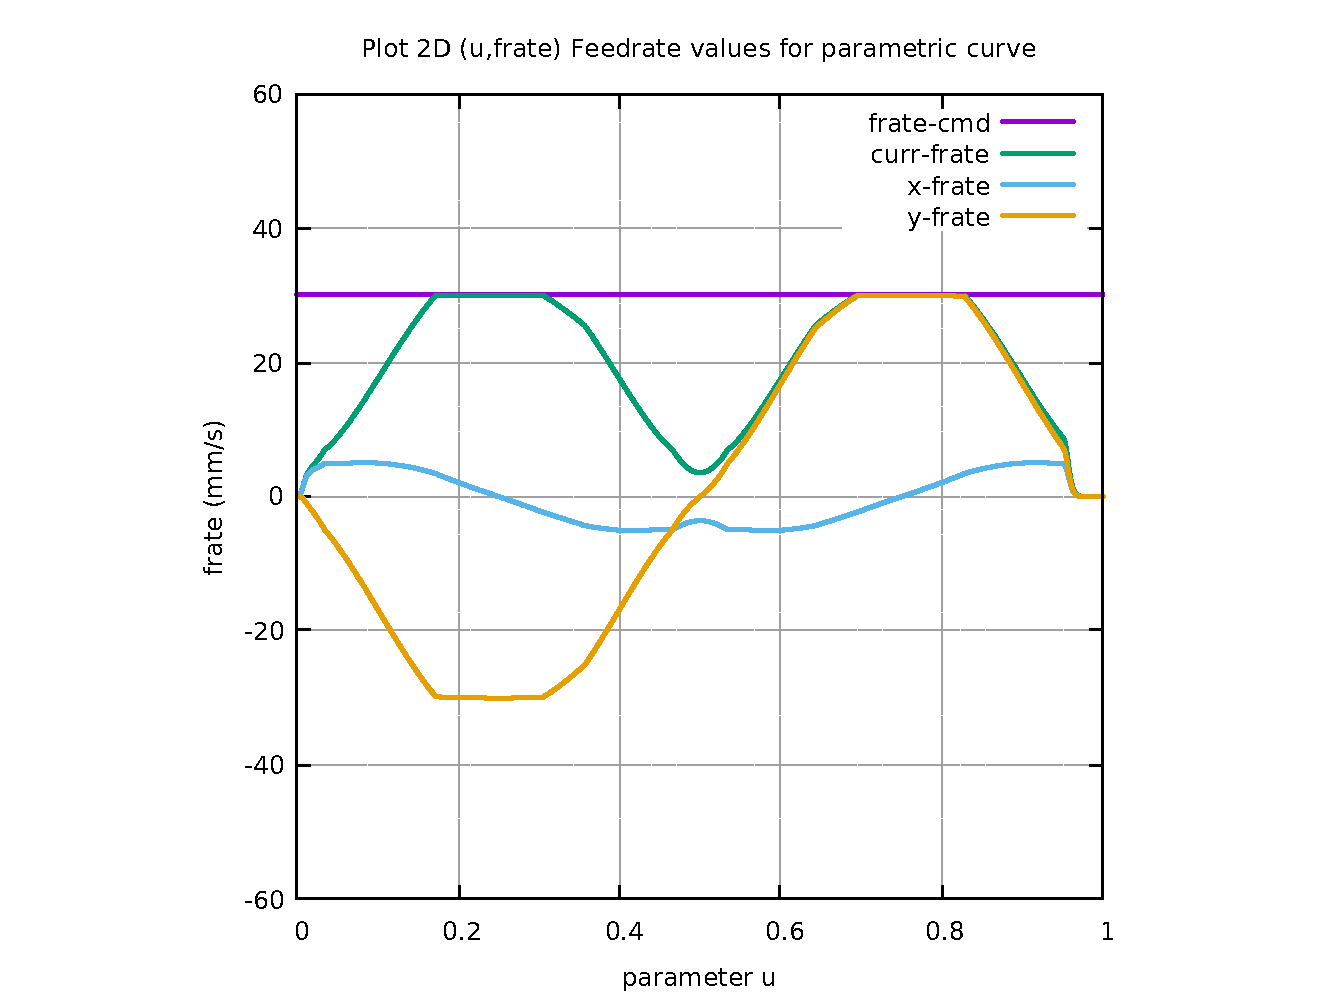
\includegraphics[width=1.00\textwidth]{Chap4/appendix/app-Ellipse/plots/29-img-Ellipse-FC30-FrateCmd-CurrFrate-X-Frate-Y-Frate.pdf}
\end{figure}


\begin{figure}
	\caption     {Ellipse FC40 FrateCmd CurrFrate X-Frate Y-Frate}
	\label{30-img-Ellipse-FC40-FrateCmd-CurrFrate-X-Frate-Y-Frate.pdf}
	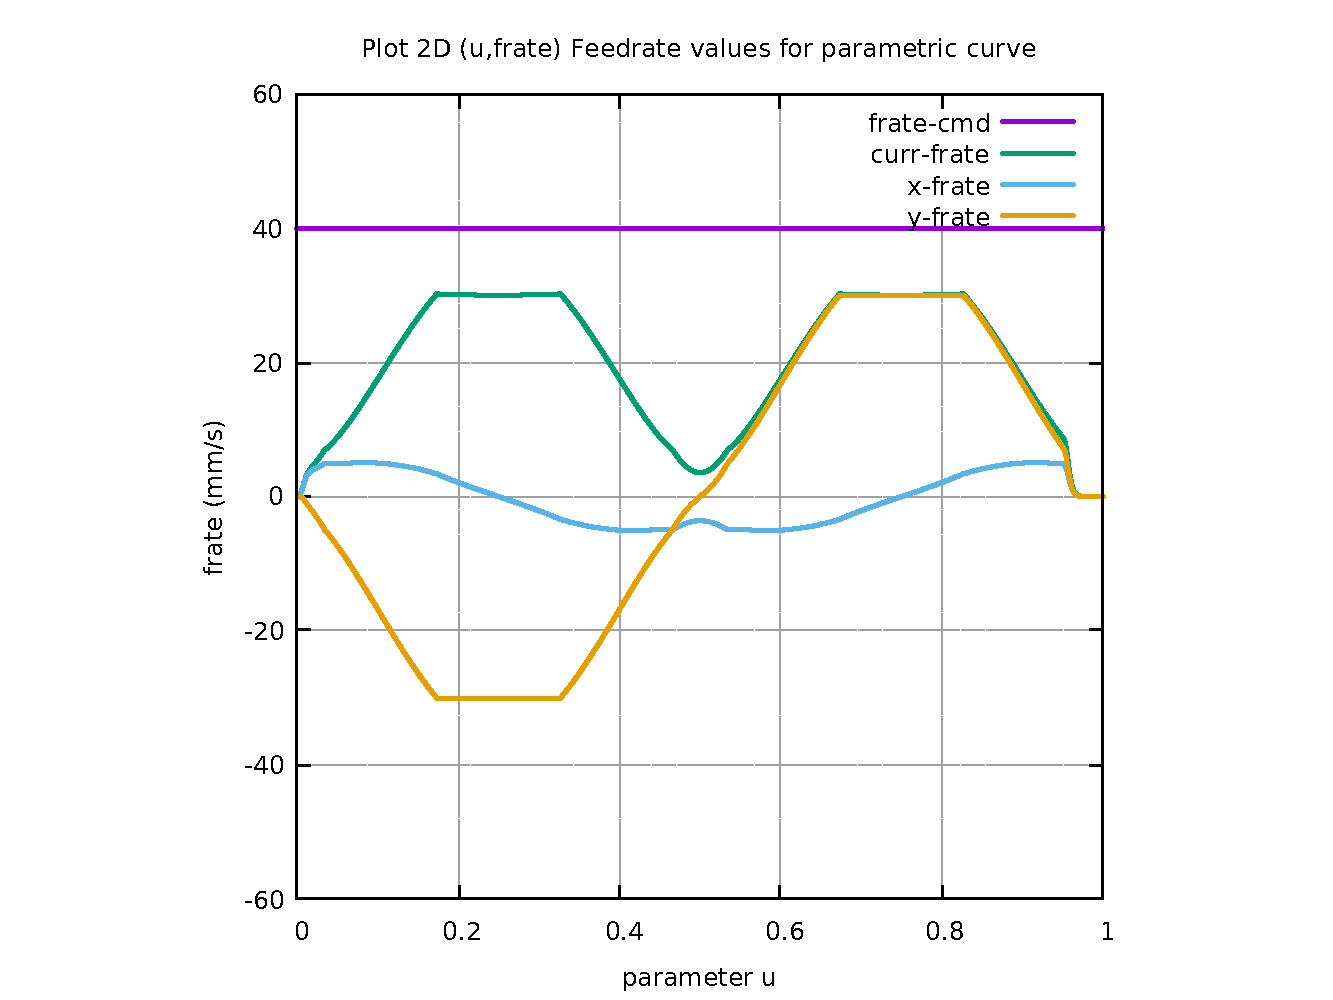
\includegraphics[width=1.00\textwidth]{Chap4/appendix/app-Ellipse/plots/30-img-Ellipse-FC40-FrateCmd-CurrFrate-X-Frate-Y-Frate.pdf}
\end{figure}


%% ==================================================
\clearpage
\pagebreak

\begin{figure}
	\caption     {Ellipse FC10 Four Components FeedrateLimit}
	\label{31-img-Ellipse-FC10-Four-Components-FeedrateLimit.pdf}
	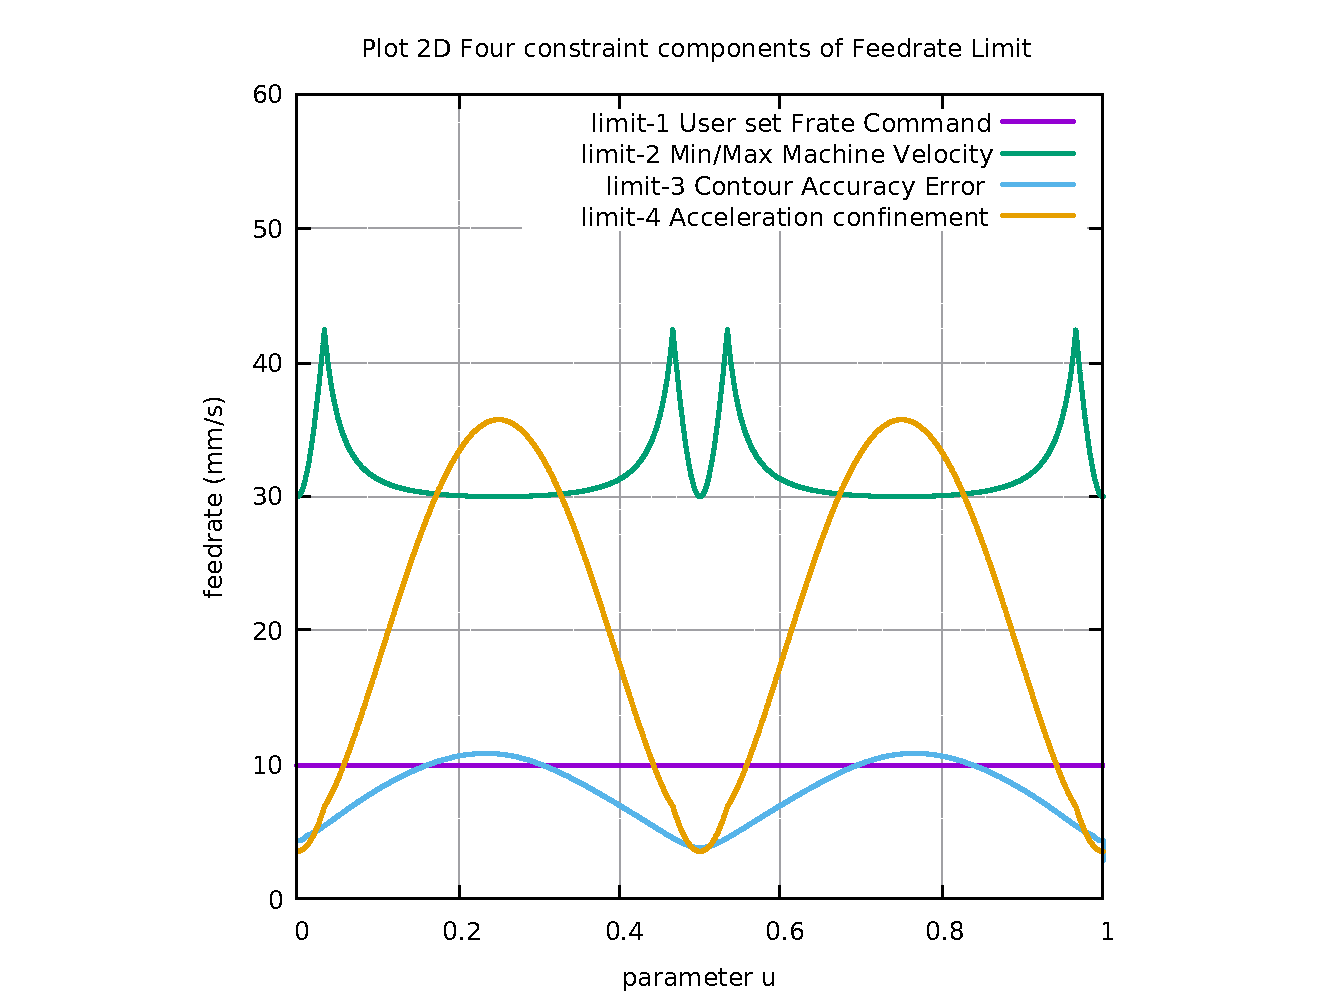
\includegraphics[width=1.00\textwidth]{Chap4/appendix/app-Ellipse/plots/31-img-Ellipse-FC10-Four-Components-FeedrateLimit.pdf}
\end{figure}


\begin{figure}
	\caption     {Ellipse FC20 Four Components FeedrateLimit}
	\label{32-img-Ellipse-FC20-Four-Components-FeedrateLimit.pdf}
	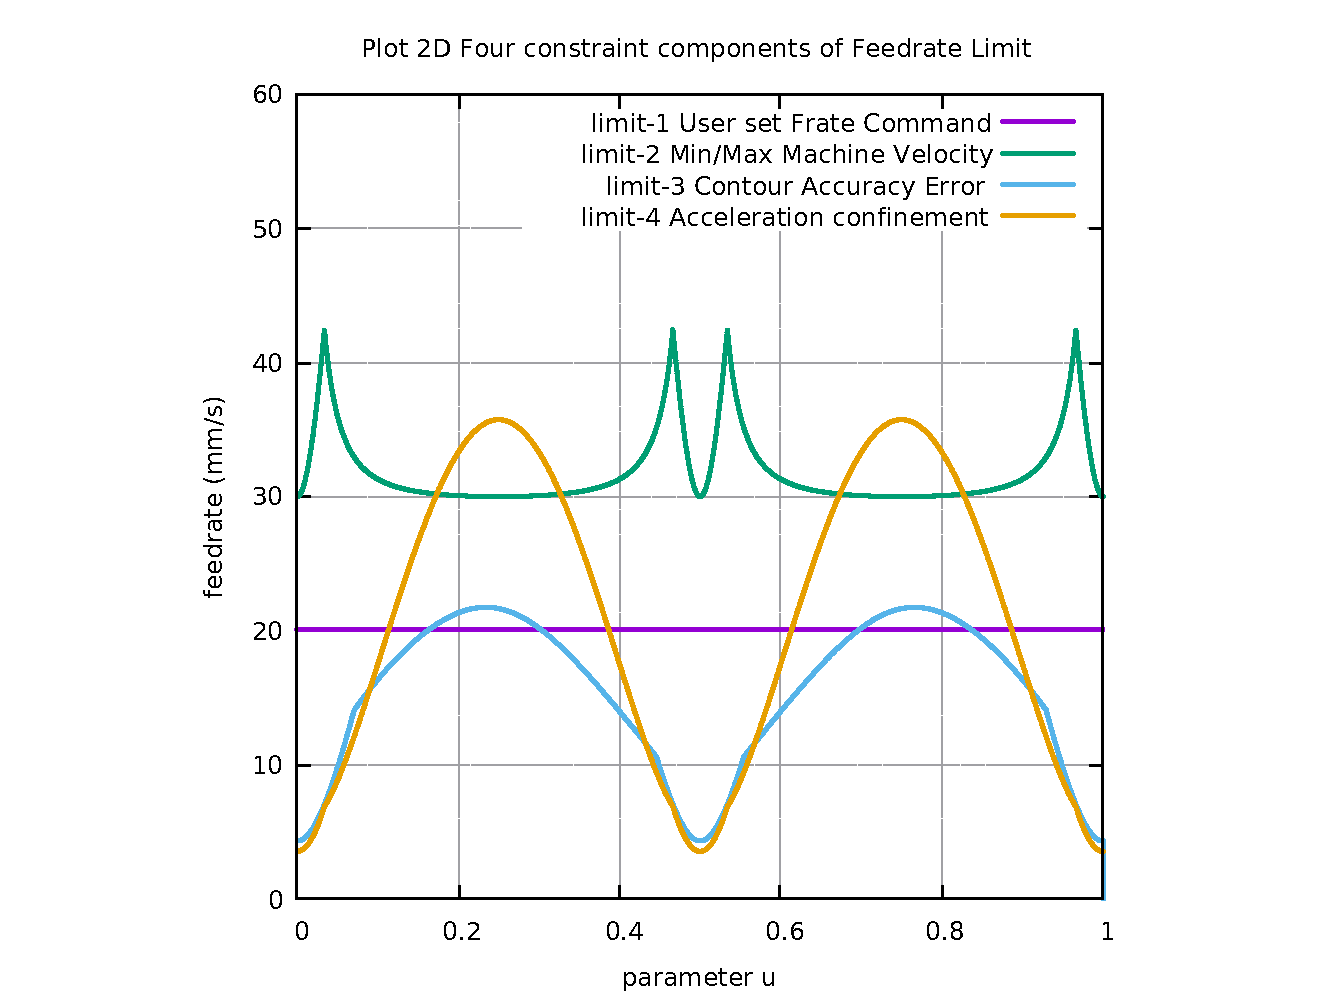
\includegraphics[width=1.00\textwidth]{Chap4/appendix/app-Ellipse/plots/32-img-Ellipse-FC20-Four-Components-FeedrateLimit.pdf}
\end{figure}


%% ==================================================
\clearpage
\pagebreak

\begin{figure}
	\caption     {Ellipse FC30 Four Components FeedrateLimit}
	\label{33-img-Ellipse-FC30-Four-Components-FeedrateLimit.pdf}
	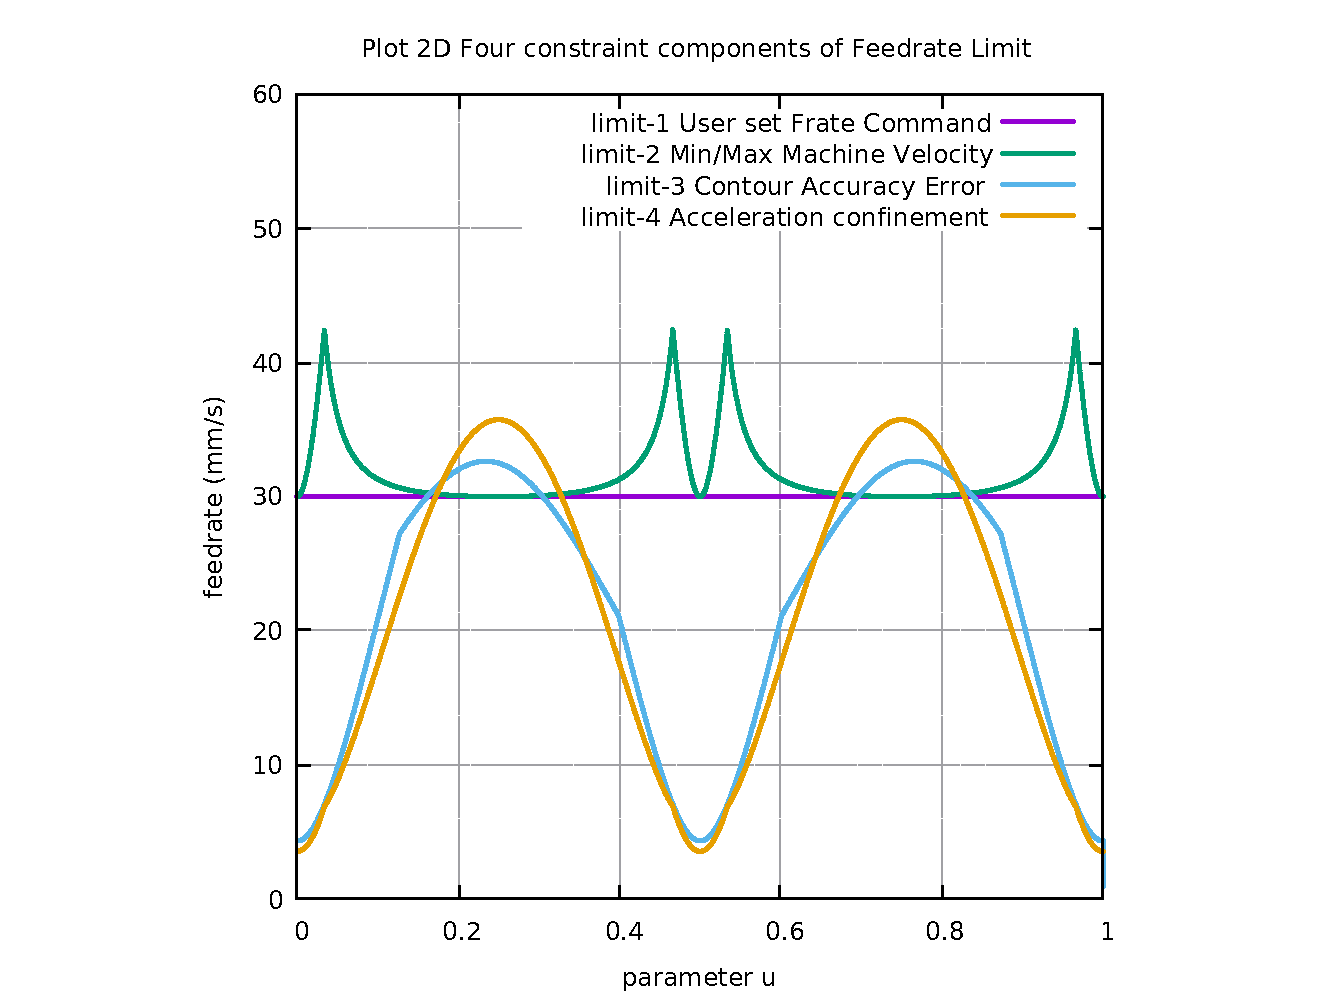
\includegraphics[width=1.00\textwidth]{Chap4/appendix/app-Ellipse/plots/33-img-Ellipse-FC30-Four-Components-FeedrateLimit.pdf}
\end{figure}


\begin{figure}
	\caption     {Ellipse FC40 Four Components FeedrateLimit}
	\label{34-img-Ellipse-FC40-Four-Components-FeedrateLimit.pdf}
	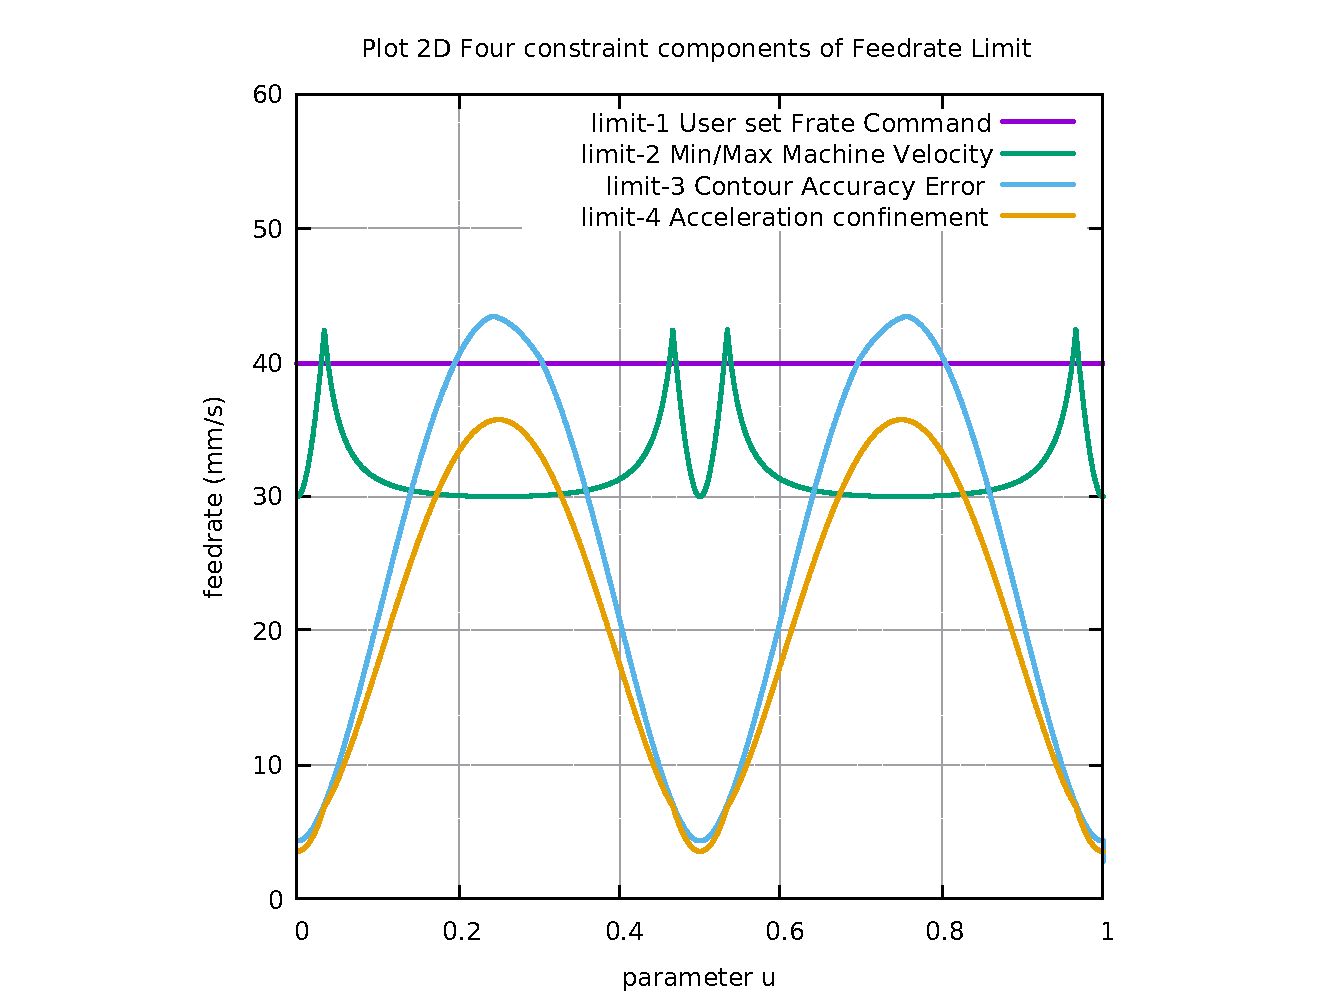
\includegraphics[width=1.00\textwidth]{Chap4/appendix/app-Ellipse/plots/34-img-Ellipse-FC40-Four-Components-FeedrateLimit.pdf}
\end{figure}


%% =======================================
\clearpage
\pagebreak

\begin{figure}
	\centering
	\caption     {Ellipse Histogram Points FC10 FC20 FC30 FC40}
	\label{35-img-Ellipse-Histogram-Points-FC10-FC20-FC30-FC40.pdf}
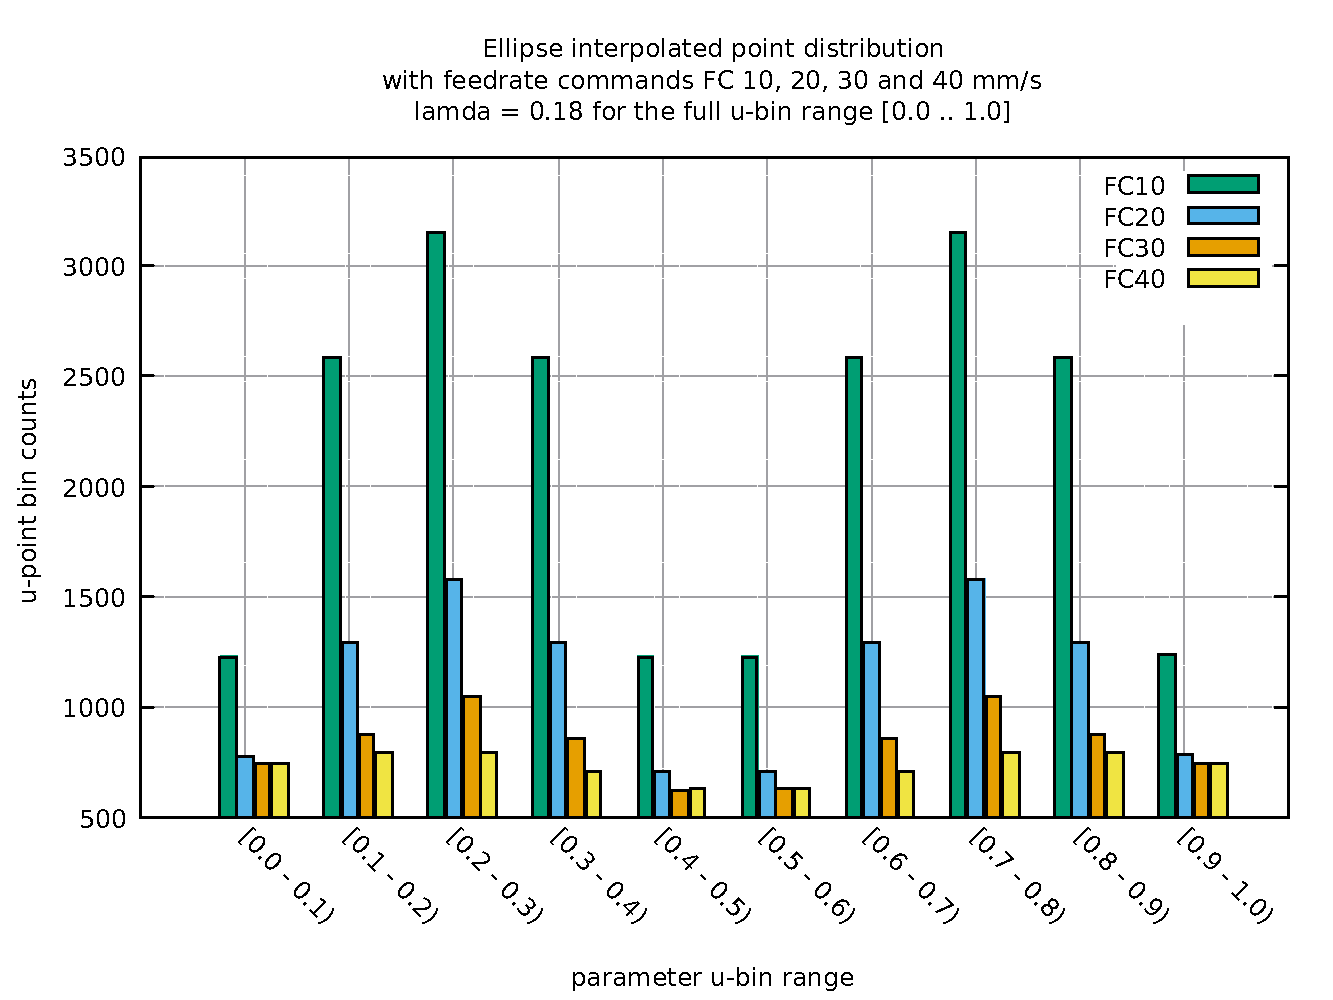
\includegraphics[width=1.00\textwidth]{Chap4/appendix/app-Ellipse/plots/35-img-Ellipse-Histogram-Points-FC10-FC20-FC30-FC40.pdf} 
\end{figure}


\begin{table}[ht]
%% \begin{center}
\caption    {Ellipse Table distribution of interpolated points}
\label  {tab-Ellipse Table distribution of interpolated points}
	
%% IMPORTANT TO SCALEBOX BELOW
\scalebox{0.80}{
		
%% START COPY AND PASTE BELOW HERE
%% FROM \begin{tabular} UNTIL \end{tabular)
%% Note: adjust last p{} to get line width correct
		
\begin{tabular}{ p{4.5cm} p{1.5cm} p{1.5cm} p{1.5cm} p{7.50cm} }
\hline
	&		&		&		&		\\
BINS	&	FC10	&	FC20	&	FC30	&	FC40	\\
    &		&		&		&		\\
0.0 - 0.1	&	4964	&	2482	&	1654	&	1241	\\
0.1 - 0.2	&	4964	&	2482	&	1655	&	1241	\\
0.2 - 0.3	&	4964	&	2482	&	1655	&	1241	\\
0.3 - 0.4	&	4964	&	2482	&	1655	&	1241	\\
0.4 - 0.5	&	4964	&	2482	&	1655	&	1242	\\
0.5 - 0.6	&	4964	&	2483	&	1655	&	1241	\\
0.6 - 0.7	&	4964	&	2482	&	1655	&	1241	\\
0.7 - 0.8	&	4964	&	2482	&	1655	&	1241	\\
0.8 - 0.9	&	4964	&	2482	&	1654	&	1242	\\
0.9 - 1.0	&	4965	&	2483	&	1656	&	1242	\\
&		&		&		&		\\
Tot Counts	&	49641	&	24822	&	16549	&	12413	\\
&		&		&		&		\\
\hline	
\end{tabular}
		
%% END COPY AND PASTE ABOVE HERE
		
}   %% IMPORTANT FOR SCALEBOX CLOSING
	
\hrule
\end{table}
%% \end{landscape}

%% ELLIPSE SUMMARY TABLE
%% ========================================================
\clearpage
\pagebreak
\begin{landscape}
	
\begin{table}[ht]
%% \begin{center}
\caption       {Ellipse Table FC10-20-30-40 Run Performance data}
\label{tab-app4-Ellipse-Table-FC10-20-30-40-Run-Performance-data}

%% IMPORTANT TO SCALEBOX BELOW
\scalebox{0.90}{
			
%% START COPY AND PASTE BELOW HERE
%% FROM \begin{tabular} UNTIL \end{tabular)
			
\begin{tabular}{ p{0.2cm} p{8.80cm} p{4.00cm} p{4.0cm} p{4.00cm} p{4.0cm}}
\hline
				&		&		&		&		&		\\
				1	&	Curve Type	&	ELLIPSE	&	ELLIPSE	&	ELLIPSE	&	ELLIPSE	\\
				2	&	User Feedrate Command FC(mm/s)                   	&	FC10	&	FC20	&	FC30	&	FC40	\\
				3	&	User Lamda Acceleration Safety Factor	&	0.18	&	0.18	&	0.18	&	0.18	\\
				&		&		&		&		&		\\
				4	&	Total Iterpolated Points (TIP)	&	21575	&	11296	&	8338	&	7351	\\
				5	&	Total Sum-Chord-Error (SCE) (mm)	&	2.990951697698E-03	&	5.148661124856E-03	&	6.561982225601E-03	&	7.331840610025E-03	\\
				6	&	Ratio 1 = (SCE/TIP) = Chord-Error/Point	&	1.386368637108E-07	&	4.558354249540E-07	&	7.870915467915E-07	&	9.975293346972E-07	\\
				&		&		&		&		&		\\
				7	&	Total Sum-Arc-Length (SAL) (mm)	&	2.156436635306E+02	&	2.156499394203E+02	&	2.156478495089E+02	&	2.156438658943E+02	\\
				8	&	Total Sum-Chord-Length (SCL) (mm)	&	2.156436625529E+02	&	2.156499358521E+02	&	2.156478426167E+02	&	2.156438551446E+02	\\
				9	&	Difference = (SAL – SCL) (mm)	&	9.777115224097E-07	&	3.568242959773E-06	&	6.892209597709E-06	&	1.074976646009E-05	\\
				10	&	Percentage Difference = (SAL – SCL)/SAL	&	4.533921870933E-07	&	1.654645936542E-06	&	3.196048378596E-06	&	4.984962783667E-06	\\
				&		&		&		&		&		\\
				11	&	Ratio 2 = (SCE/SCL) = Chord Error/Chord-Length	&	1.386987988559E-05	&	2.387508767166E-05	&	3.042915776933E-05	&	3.399976598039E-05	\\
				&		&		&		&		&		\\
				12	&	Total Sum-Arc-Theta (SAT) (rad)	&	6.280515723261E+00	&	6.283169115421E+00	&	6.282291919271E+00	&	6.280610715483E+00	\\
				13	&	Total Sum-Arc-Area (SAA) (mm2)	&	5.185017589366E-05	&	1.275076043292E-04	&	1.849039783361E-04	&	2.200267776119E-04	\\
				&		&		&		&		&		\\
				14	&	Ratio 3 = (SAA/SCL) = Arc-Area/Chord-Length	&	1.386987988559E-05	&	2.387508767166E-05	&	3.042915776933E-05	&	3.399976598039E-05	\\
				&		&		&		&		&		\\
				15	&	Average-Chord-Error (ACE) (mm)	&	1.386368637108E-07	&	4.558354249540E-07	&	7.870915467915E-07	&	9.975293346972E-07	\\
				16	&	Average-Arc-Length (AAL) (mm)	&	9.995534603255E-03	&	1.909251345023E-02	&	2.586636074235E-02	&	2.933930148222E-02	\\
				17	&	Average-Chord-Length (ACL) (mm)	&	9.995534557936E-03	&	1.909251313431E-02	&	2.586635991565E-02	&	2.933930001967E-02	\\
				18	&	Average-Arc-Theta (AAT) (rad)	&	2.911150330611E-04	&	5.562788061462E-04	&	7.535434711852E-04	&	8.545048592494E-04	\\
				19	&	Average-Arc-Area (AAA) (mm2)	&	2.403364044390E-09	&	1.128885385827E-08	&	2.217871876407E-08	&	2.993561600162E-08	\\
				&		&		&		&		&		\\
				20	&	Algorithm actual runtime on computer (ART) (s) 	&	7.13439876	&	7.633051722	&	11.041426063	&	16.776571251	\\
				&		&		&		&		&	\\	
\hline				
\end{tabular}
			
%% END COPY AND PASTE		
}   %% IMPORTANT FOR SCALEBOX CLOSING

\end{table}
\end{landscape}

%% =======================================
\clearpage
\pagebreak
